\documentclass[../Bachelorarbeit.tex]{subfiles}

\begin{document}
\label{sec:results}
The \acrshort{eft} samples for each parameter S0, M0, M1, T0, T1, T2 are fitted against the combined \acrshort{sm} and \acrshort{gm} Resonance data. It is assumed that the coefficients are only affected by anomalous \acrshort{qgc} (aQGC) couplings.
Only one coefficient is fitted at once while the other coefficients are set to zero. As discussed in section \ref{sec:EFT} good fits are expected for sufficiently high resonance mass.
The fit can't identify small energies or high energy with small cross-sections resonances as shown in \ref{fig:S1_with_fit_diffrence_225}\footnote{Technical reasons cause the ratio plot to display the wrong errors}.

\begin{figure}[h]
    \centering
    \begin{subfigure}{0.3\textwidth}
        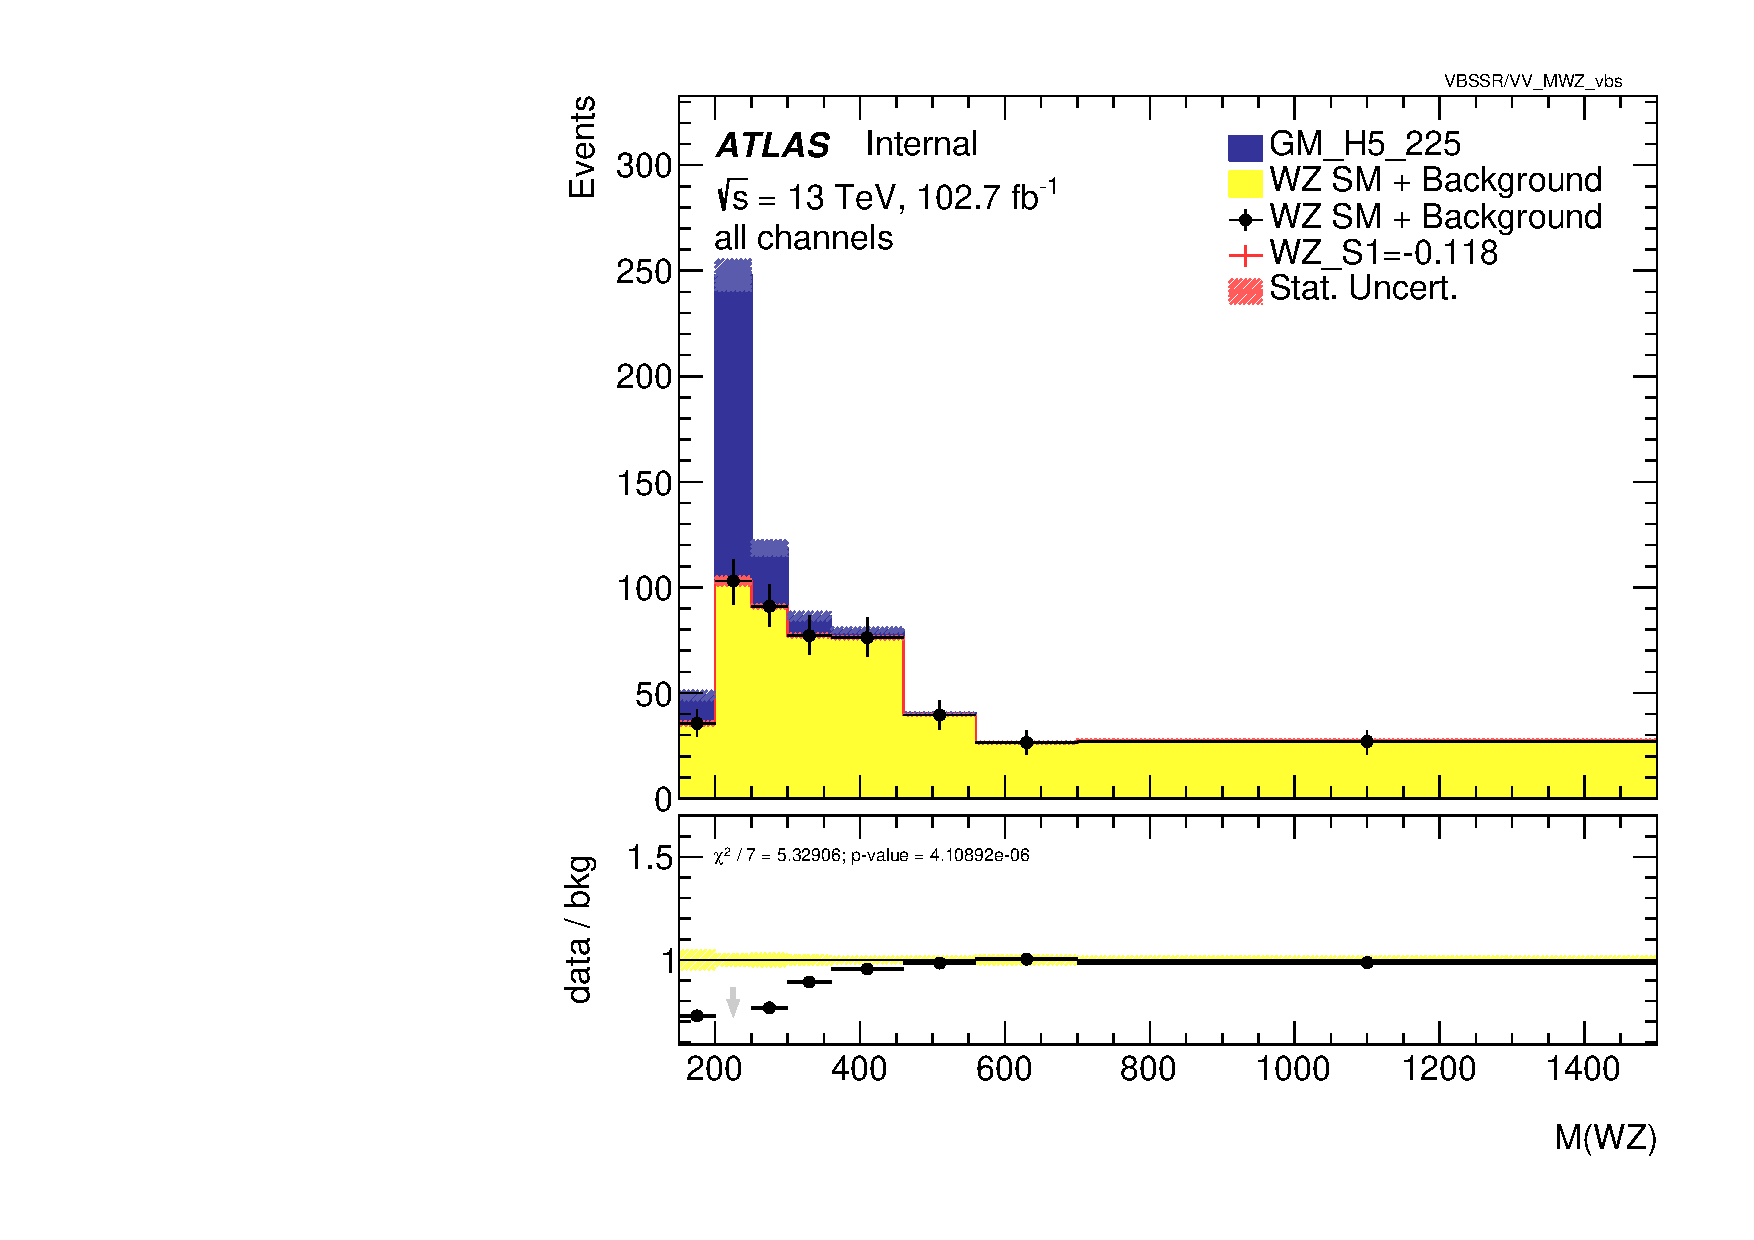
\includegraphics[width=\textwidth]{Plots/ALL_MWZ_right_color/GM_H5_225/S1/2022-05-07/VBSSR/all_VV_MWZ_vbs.pdf}
        \caption{}
    \end{subfigure}
    \begin{subfigure}{0.3\textwidth}
        \includegraphics[width=\textwidth]{Plots/ALL_MWZ_right_color/GM_H5_800/S1/2022-05-07/VBSSR/all_VV_MWZ_vbs.pdf}
        \caption{}
    \end{subfigure}
    \begin{subfigure}{0.3\textwidth}
        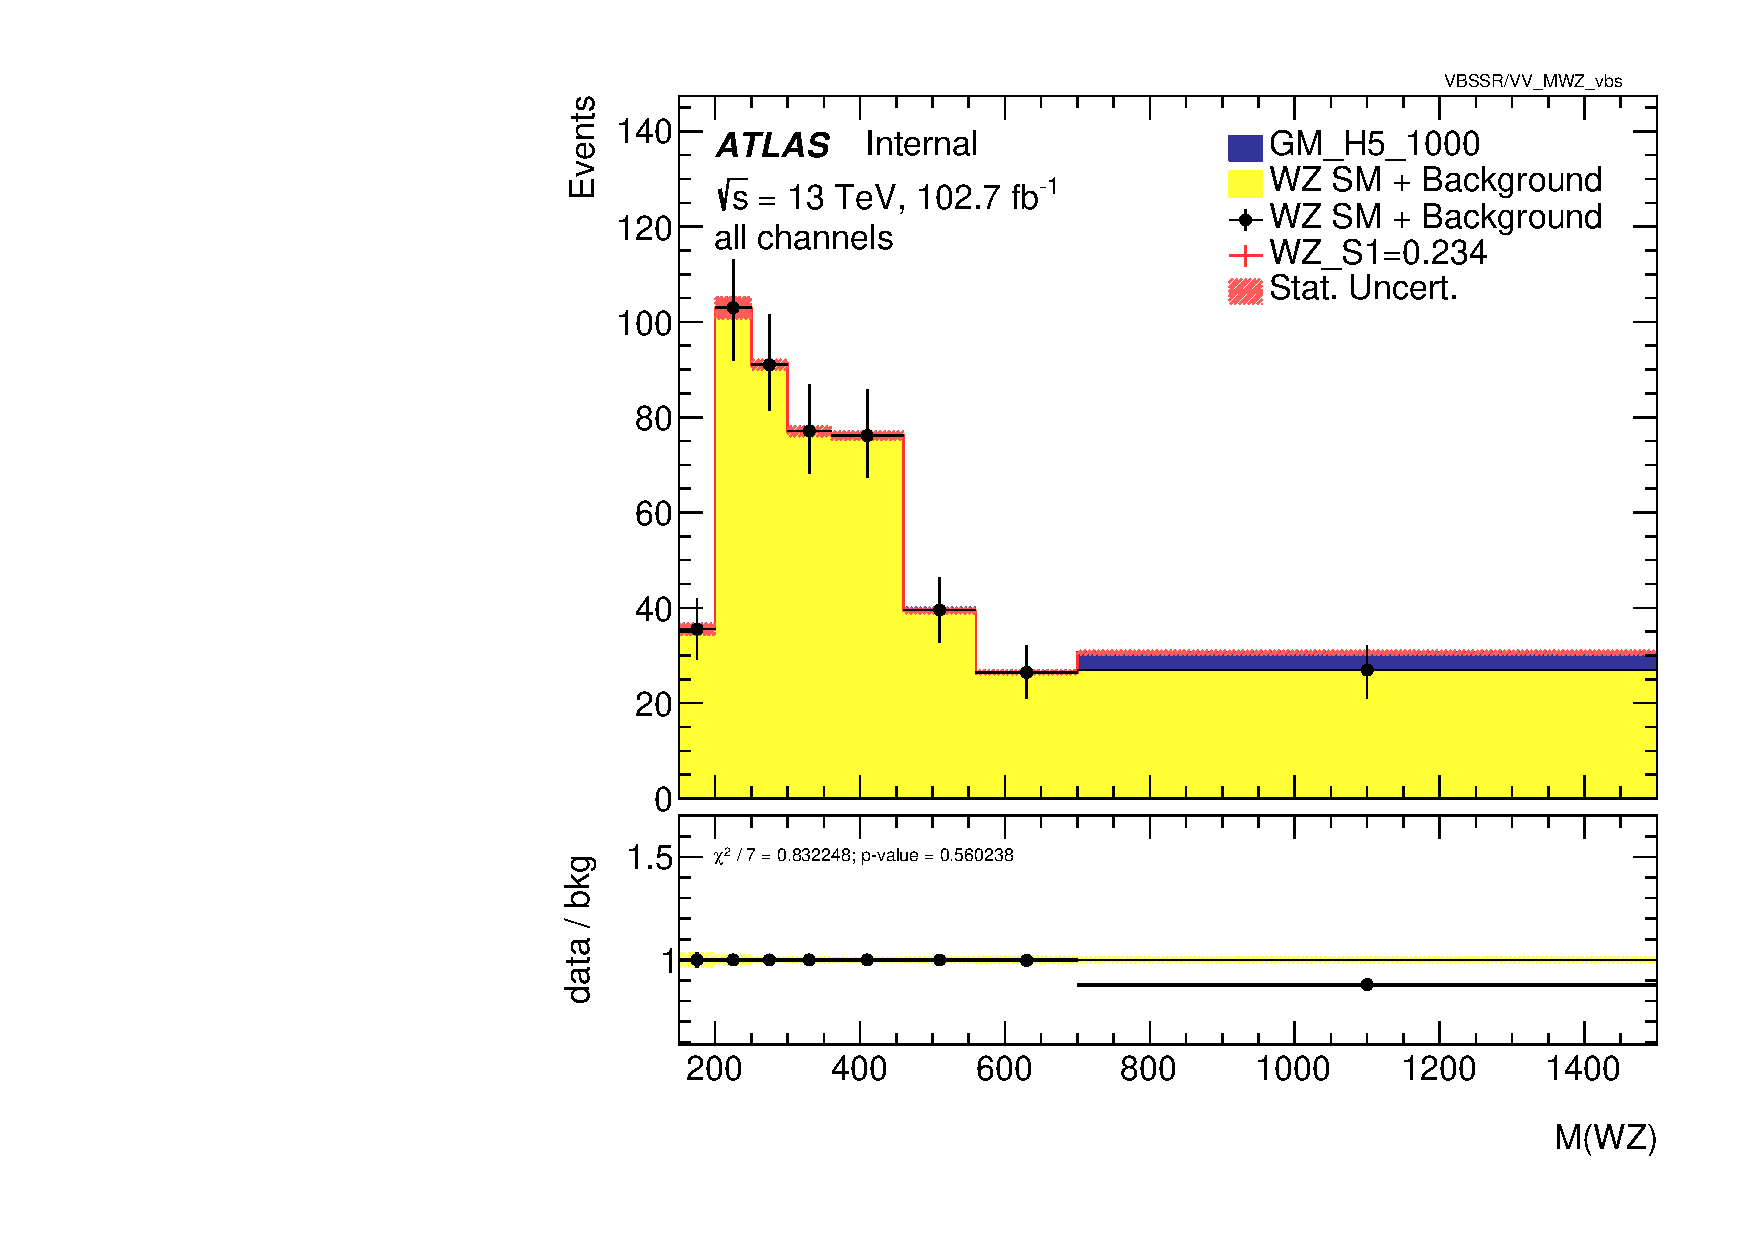
\includegraphics[width=\textwidth]{Plots/05x_for_comparision/VBSSR/all_VV_MWZ_vbs.pdf}
        \caption{}
    \end{subfigure}
    \caption{\textbf{a)}The invariant Mass of the resonance has approximately the same energy as the WZ peak but for the WZ peak the \acrshort{eft} prediction
        should be the \acrshort{sm} therefore \acrshort{eft} can't describe the 225 GeV Resonance and the coefficient fit diverges.
        \textbf{b)}800 GeV has a high cross-section and the energy is in the region where \acrshort{sm} and \acrshort{eft} deviate therefore the coefficients can be fitted accurately.
        \textbf{c)}1000 GeV the cross-section(scaled by 0.5) is to low the fit can produce a significant result even though the Resonance is in the right Energy region.}
    \label{fig:S1_with_fit_diffrence_225}
\end{figure}
Evaluating which fit is good can be done qualitative by simply looking at the invariant mass plots if the \acrshort{eft} sample scaled with the best fit value is able to describe
the resonance one can argue that the fit is good. But this is not accurately possible for resonances peaks that are higher energy than the $W^{\pm}Z$ peak, but the start of the peak is still part of the $W^{\pm}Z$ peak.\\\\
For a quantitative analysis the significance quotient has to be calculated from the likelihood ratio $f(\mu)=-2\Delta log(L)$ where $\mu$ is the signal strength.
The significance can be calculated using $Z(\mu)=\sqrt{f(\mu)}$ resulting in $S = \frac{Z_{GM}(0)}{Z_{EFT}(0)}$.
Here $Z_{GM}$ is the significance when the \acrshort{gm} sample is used as coefficient in \acrshort{eft}Fun \cite{EFTfun.} and fitted with \acrshort{sm} as measurement and as prediction.
The $Z_{EFT}$ is the fit of an \acrshort{eft} coefficient for the \acrshort{sm} combined with the \acrshort{gm} model as measurement against the \acrshort{sm} as prediction.
$f(0)$ can be interpreted as the difference to the \acrshort{sm}, if $f(0) = 0$ only the \acrshort{sm} was measured. If $f(0)>0$ there is an \acrshort{eft}, \acrshort{gm} which is more likely than the \acrshort{sm}. For $f(0) > 4$ the \acrshort{sm} is excluded.
The value of $\mu=0$ can be read off from the log-likelihood ratio plot in \ref{fig:EFT_GM_Asimov_comparision}. The scale is dependent on
the operator as well as the allowed range making it difficult to estimate a read off error. The error can be minimized by looking at positive and negative extrema and limiting the range to zero as well as the shape including both extrema.
Since the likelihood-function is continuous all plots give the same $f(0)$ value. All three ranges should be used in case only an extremum exists, or only one is recognized by the fit this is often the case for low energy resonances.
Using this the error becomes small compared to the statistical errors. All \acrshort{eft} coefficients in \ref{fig:significans_plots} with $S>0.8$ are able to reproduce the statistical significance of the \acrshort{gm} model to more than $80\%$ certainty.
\begin{figure}[h]
    \centering
    \begin{subfigure}{0.3\textwidth}
        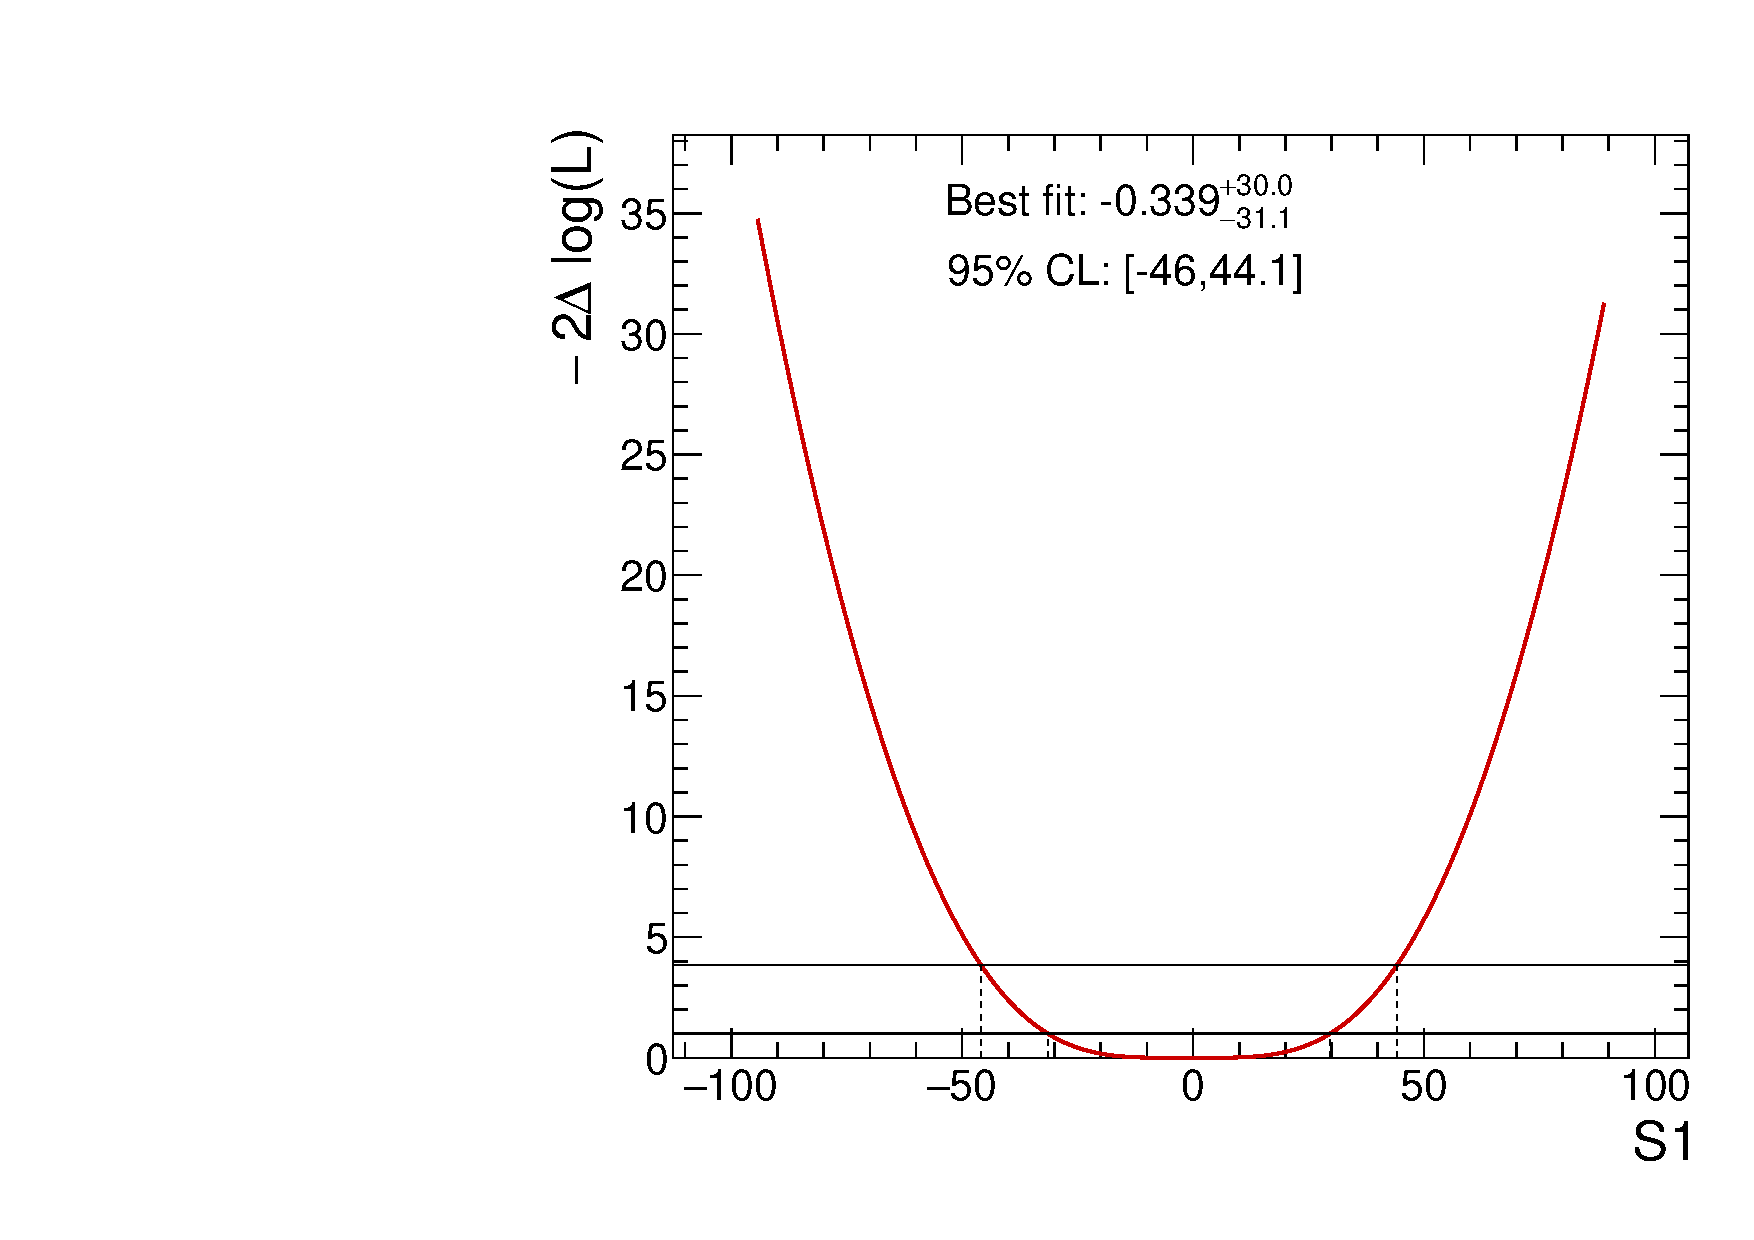
\includegraphics[width=\textwidth]{Plots/operators/S1_asimov.pdf}
        \caption{S1 Asmiov fit}
    \end{subfigure}
    \begin{subfigure}{0.3\textwidth}
        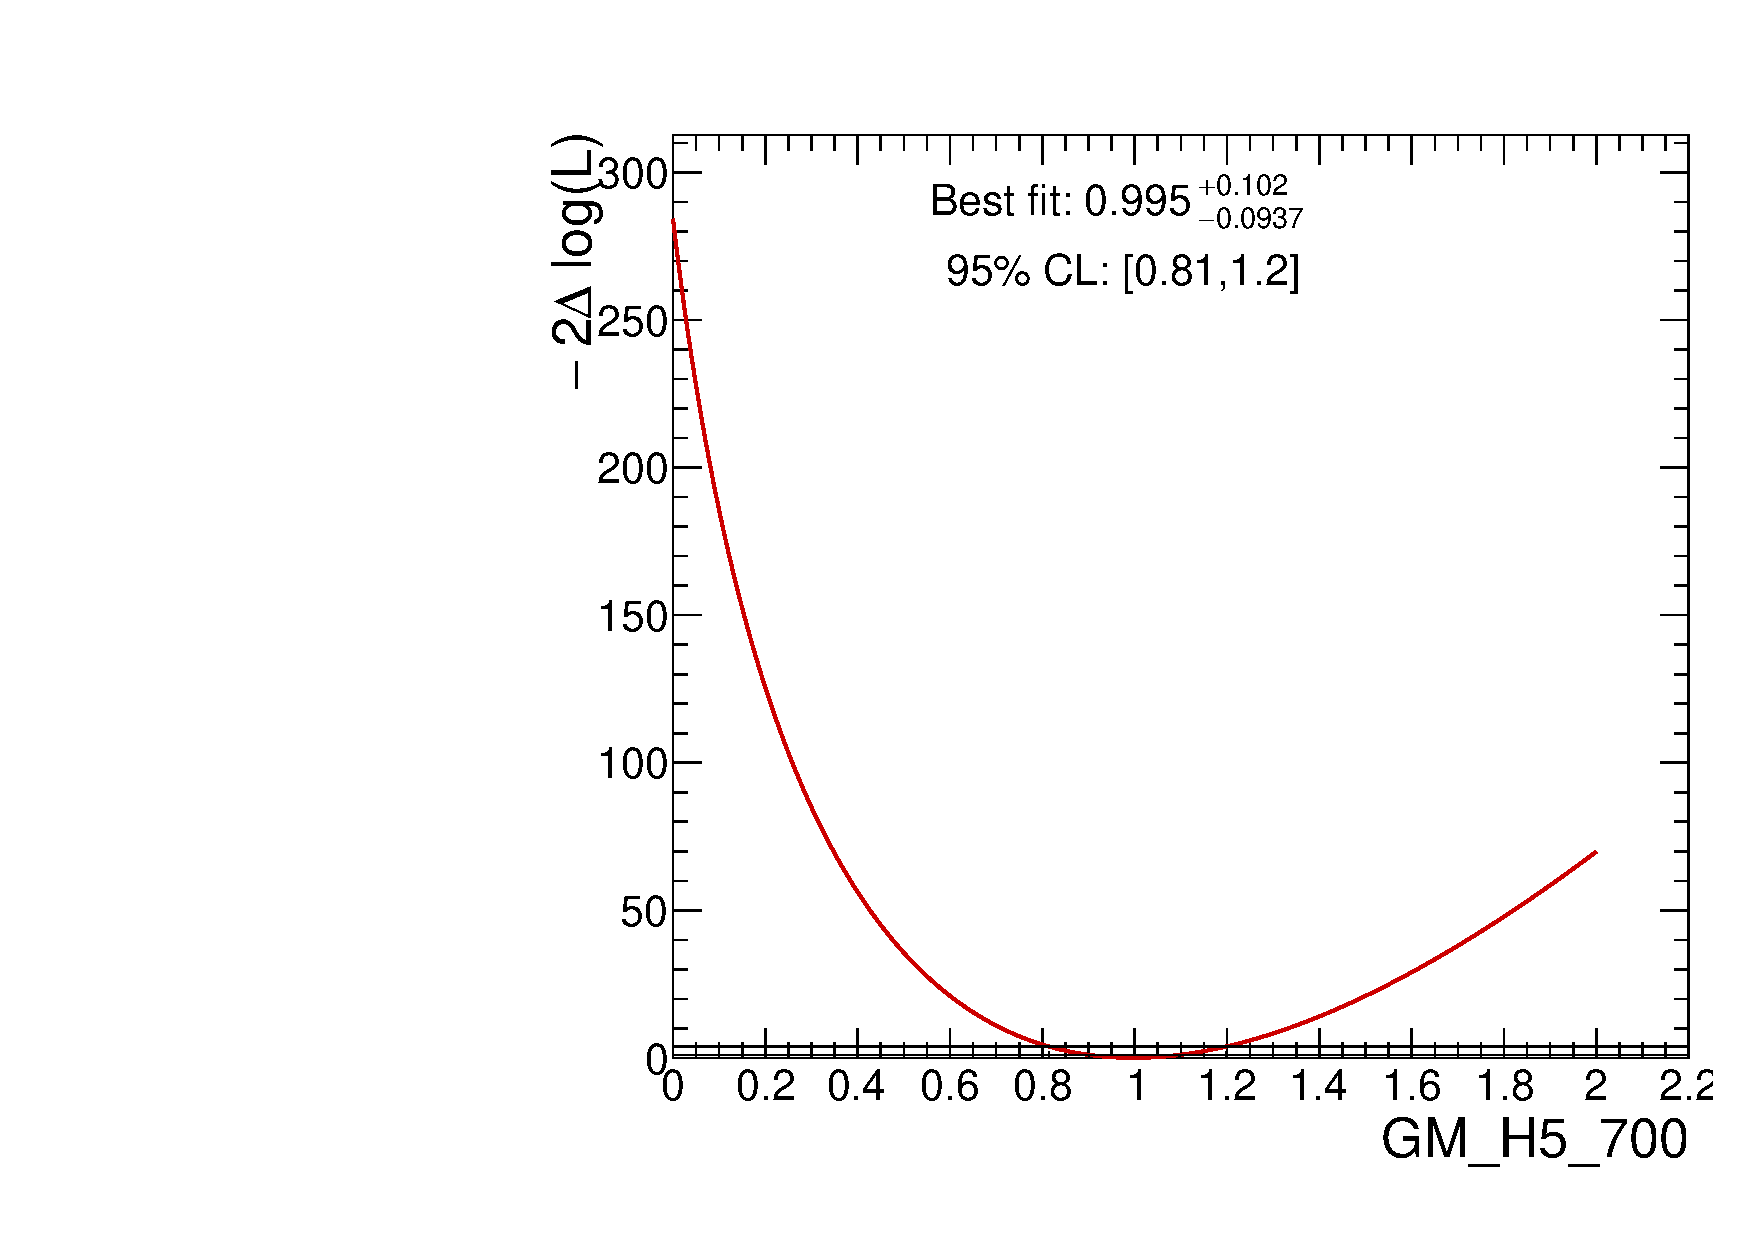
\includegraphics[width=\textwidth]{Plots/operators/GM_H5_700_scan_coef.pdf}
        \caption{700 GeV GM}
    \end{subfigure}
    \begin{subfigure}{0.3\textwidth}
        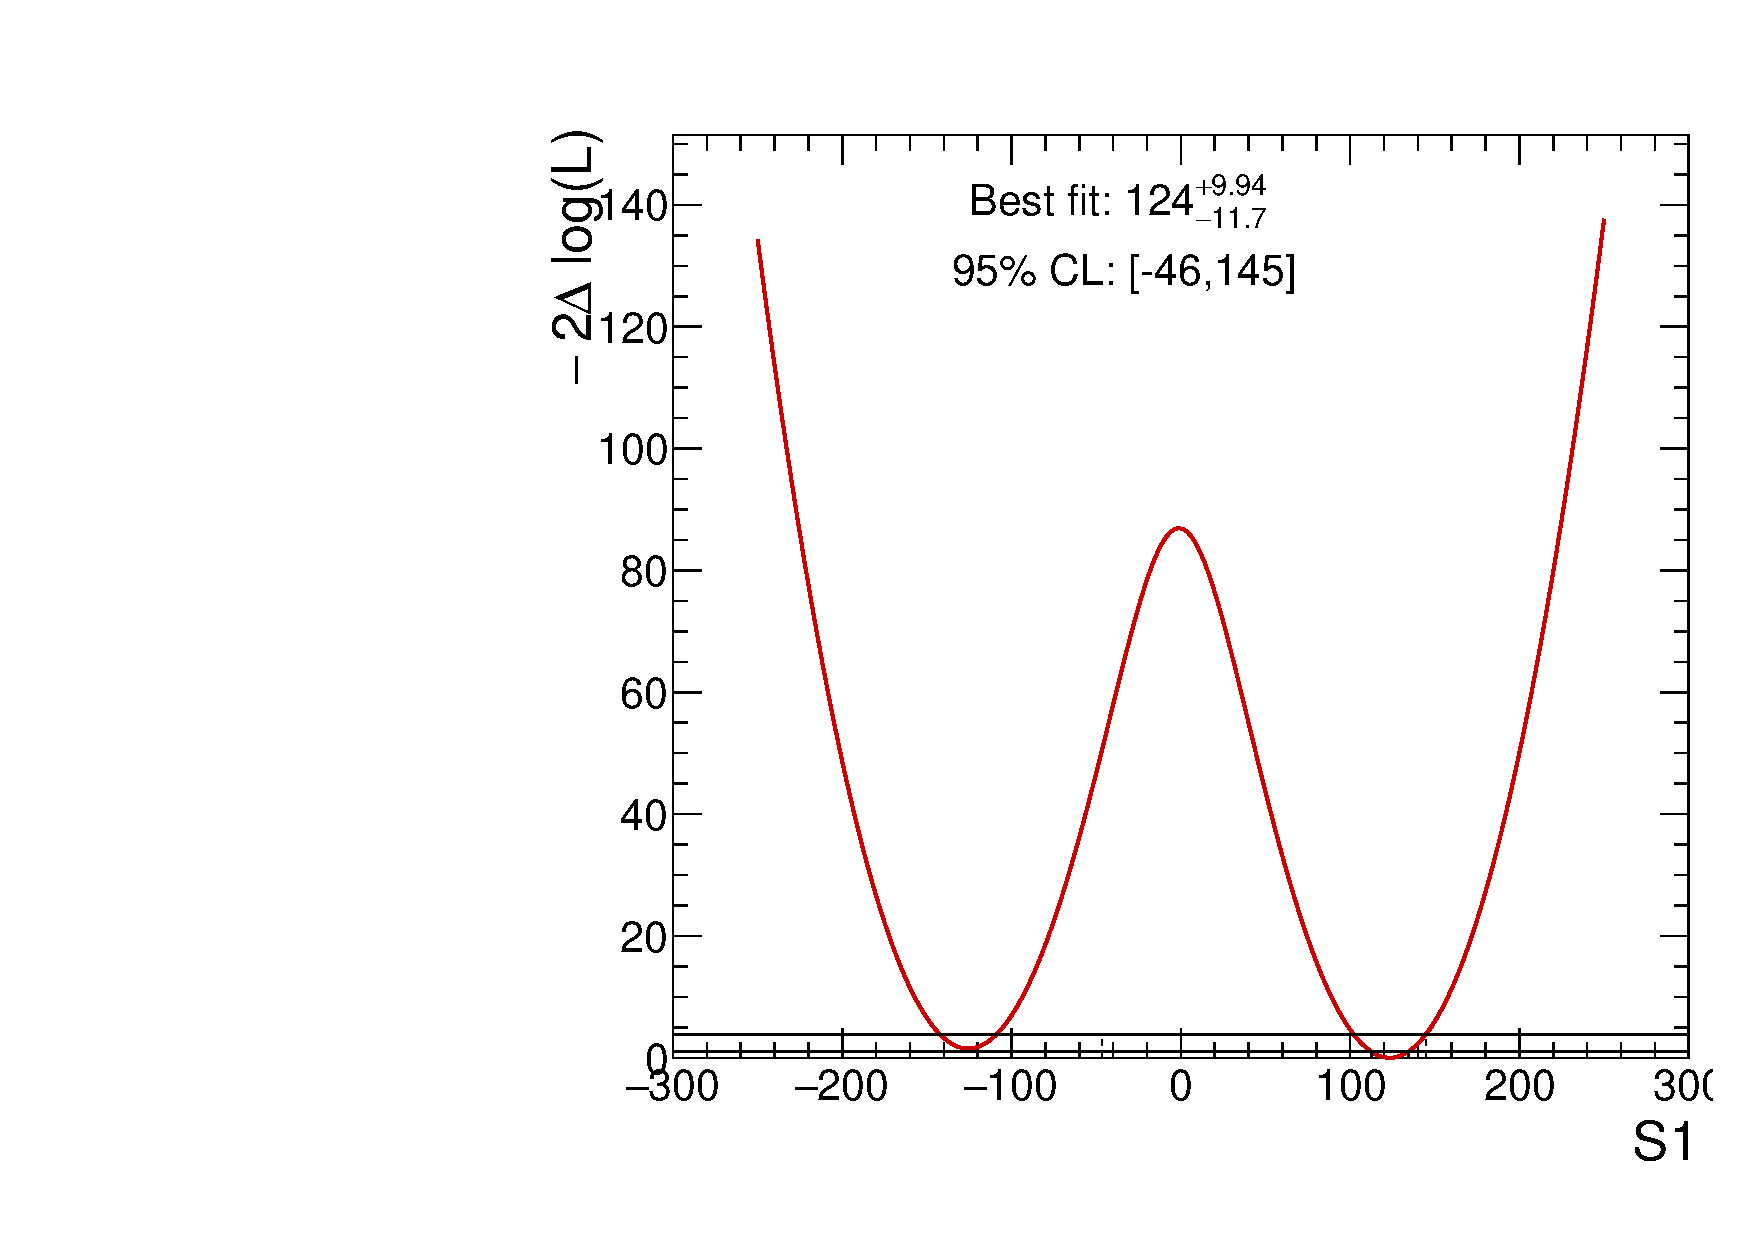
\includegraphics[width=\textwidth]{Plots/operators/S1_EFT.pdf}
        \caption{S1 for 700 GeV}
    \end{subfigure}
    \caption{\textbf{a)}The best fit value is zero since the \acrshort{sm} is reproduced in the Asimov fit.
        \textbf{c)} The \acrshort{sm} is excluded, and two extrema emerge from the inclusion of the quadratic operator therm.}
    \label{fig:EFT_GM_Asimov_comparision}
\end{figure}

\begin{figure}[h]
    \centering
    \begin{subfigure}{0.45\textwidth}
        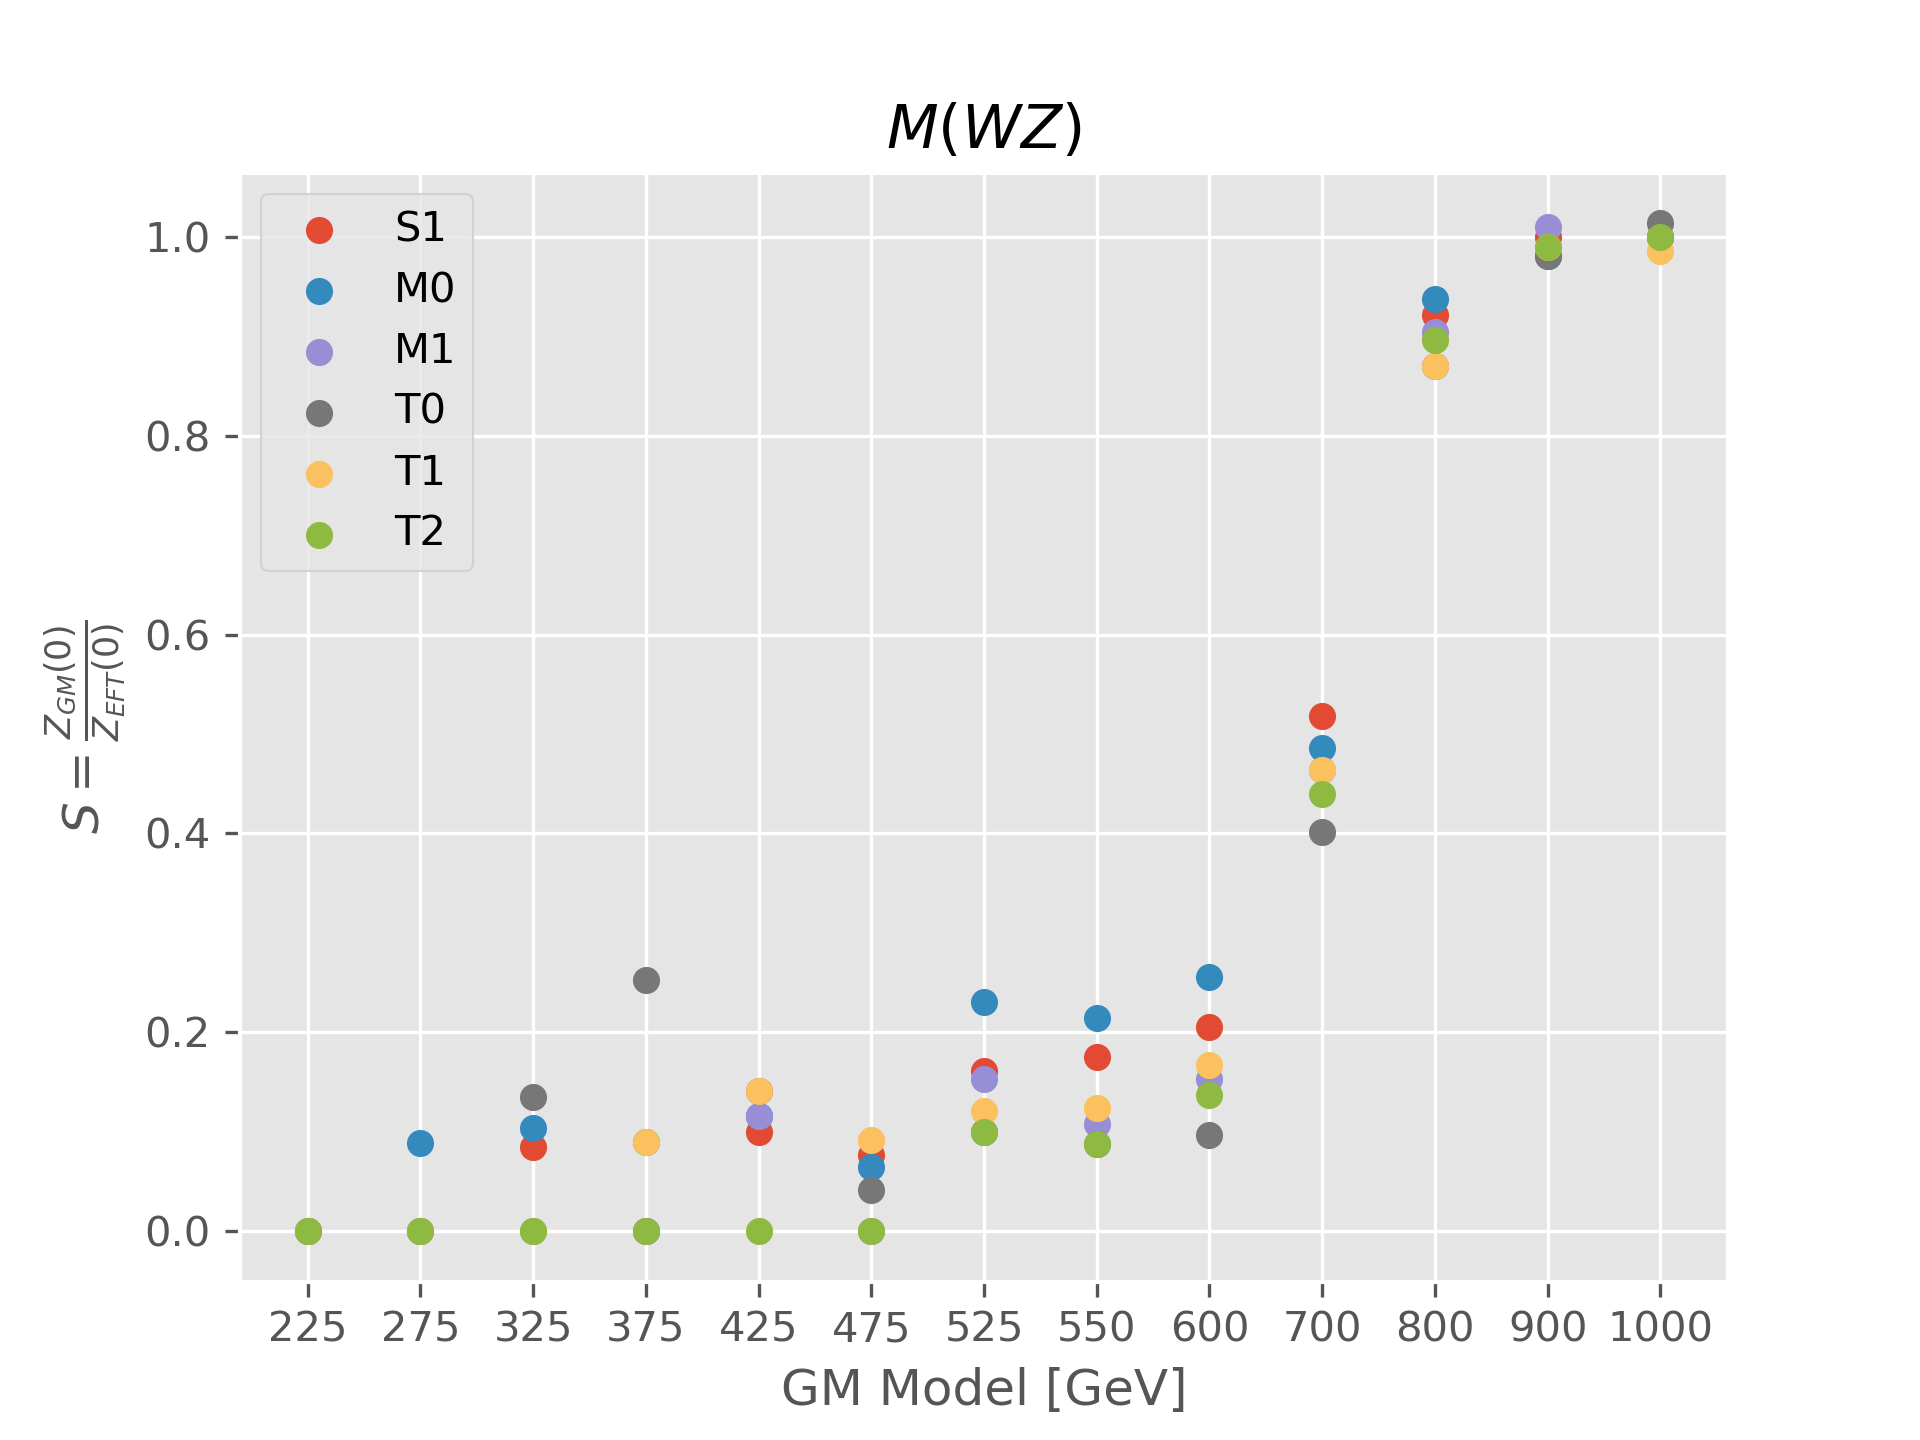
\includegraphics[width=\textwidth]{Plots/gm_relevanze/MWZ_all.png}
        \caption{}
    \end{subfigure}
    \begin{subfigure}{0.45\textwidth}
        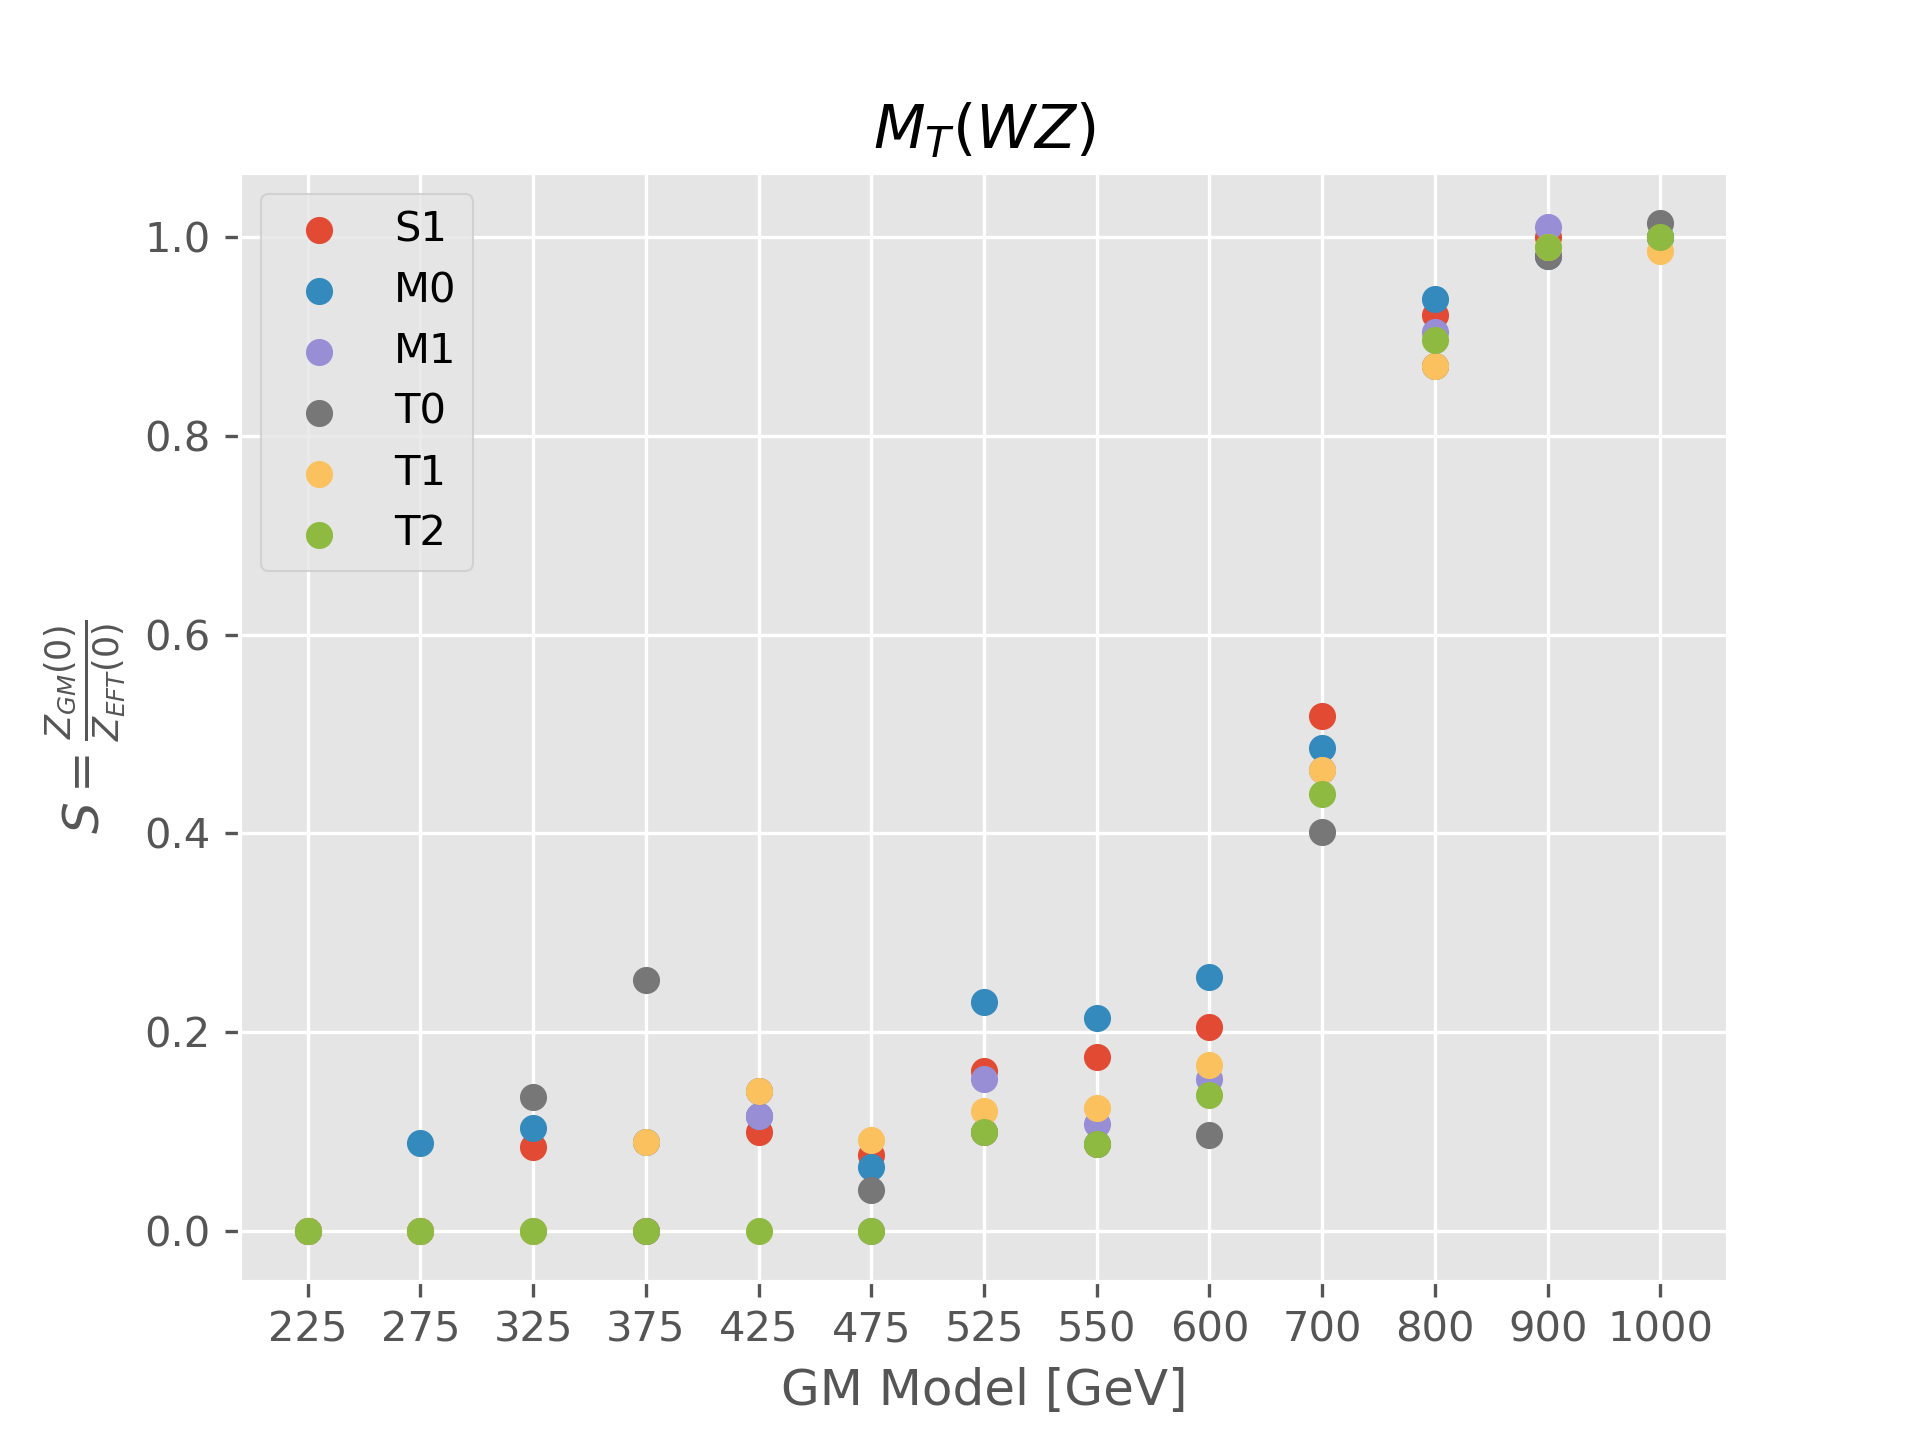
\includegraphics[width=\textwidth]{Plots/gm_relevanze/MTWZ_all.png}
        \caption{}
    \end{subfigure}
    \caption{a) \acrshort{eft} coefficients significance for invariant Mass b) \acrshort{eft} coefficients significance for transverse Mass. Plots for all operators indiviualy are shwon in appendix \ref{sec:signif_dim8}}
    \label{fig:significans_plots}
\end{figure}
\newpage
The result is independent of the resonance cross-section. This can be shown by scaling the resonance, in \ref{fig:corss-section-comparission} the cross-section is scaled with $2$ and $0.5$ which results in equal significance compared to the non-scaled resonances.
The cross-section can not be scaled higher without breaking the fitting-tool as the values get unreasonably high. In the invariant mass plot for 0.5 times the cross-section, the cross-section becomes too low to be picked up by the fitting tool. In the transverse mass plot
the resonance is shown to be picked up and described by the coefficients M0, T0, T1 this however is falls as these did not pass a qualitative analysis without scaling.
\begin{figure}[h]
    \centering
    \begin{subfigure}{0.45\textwidth}
        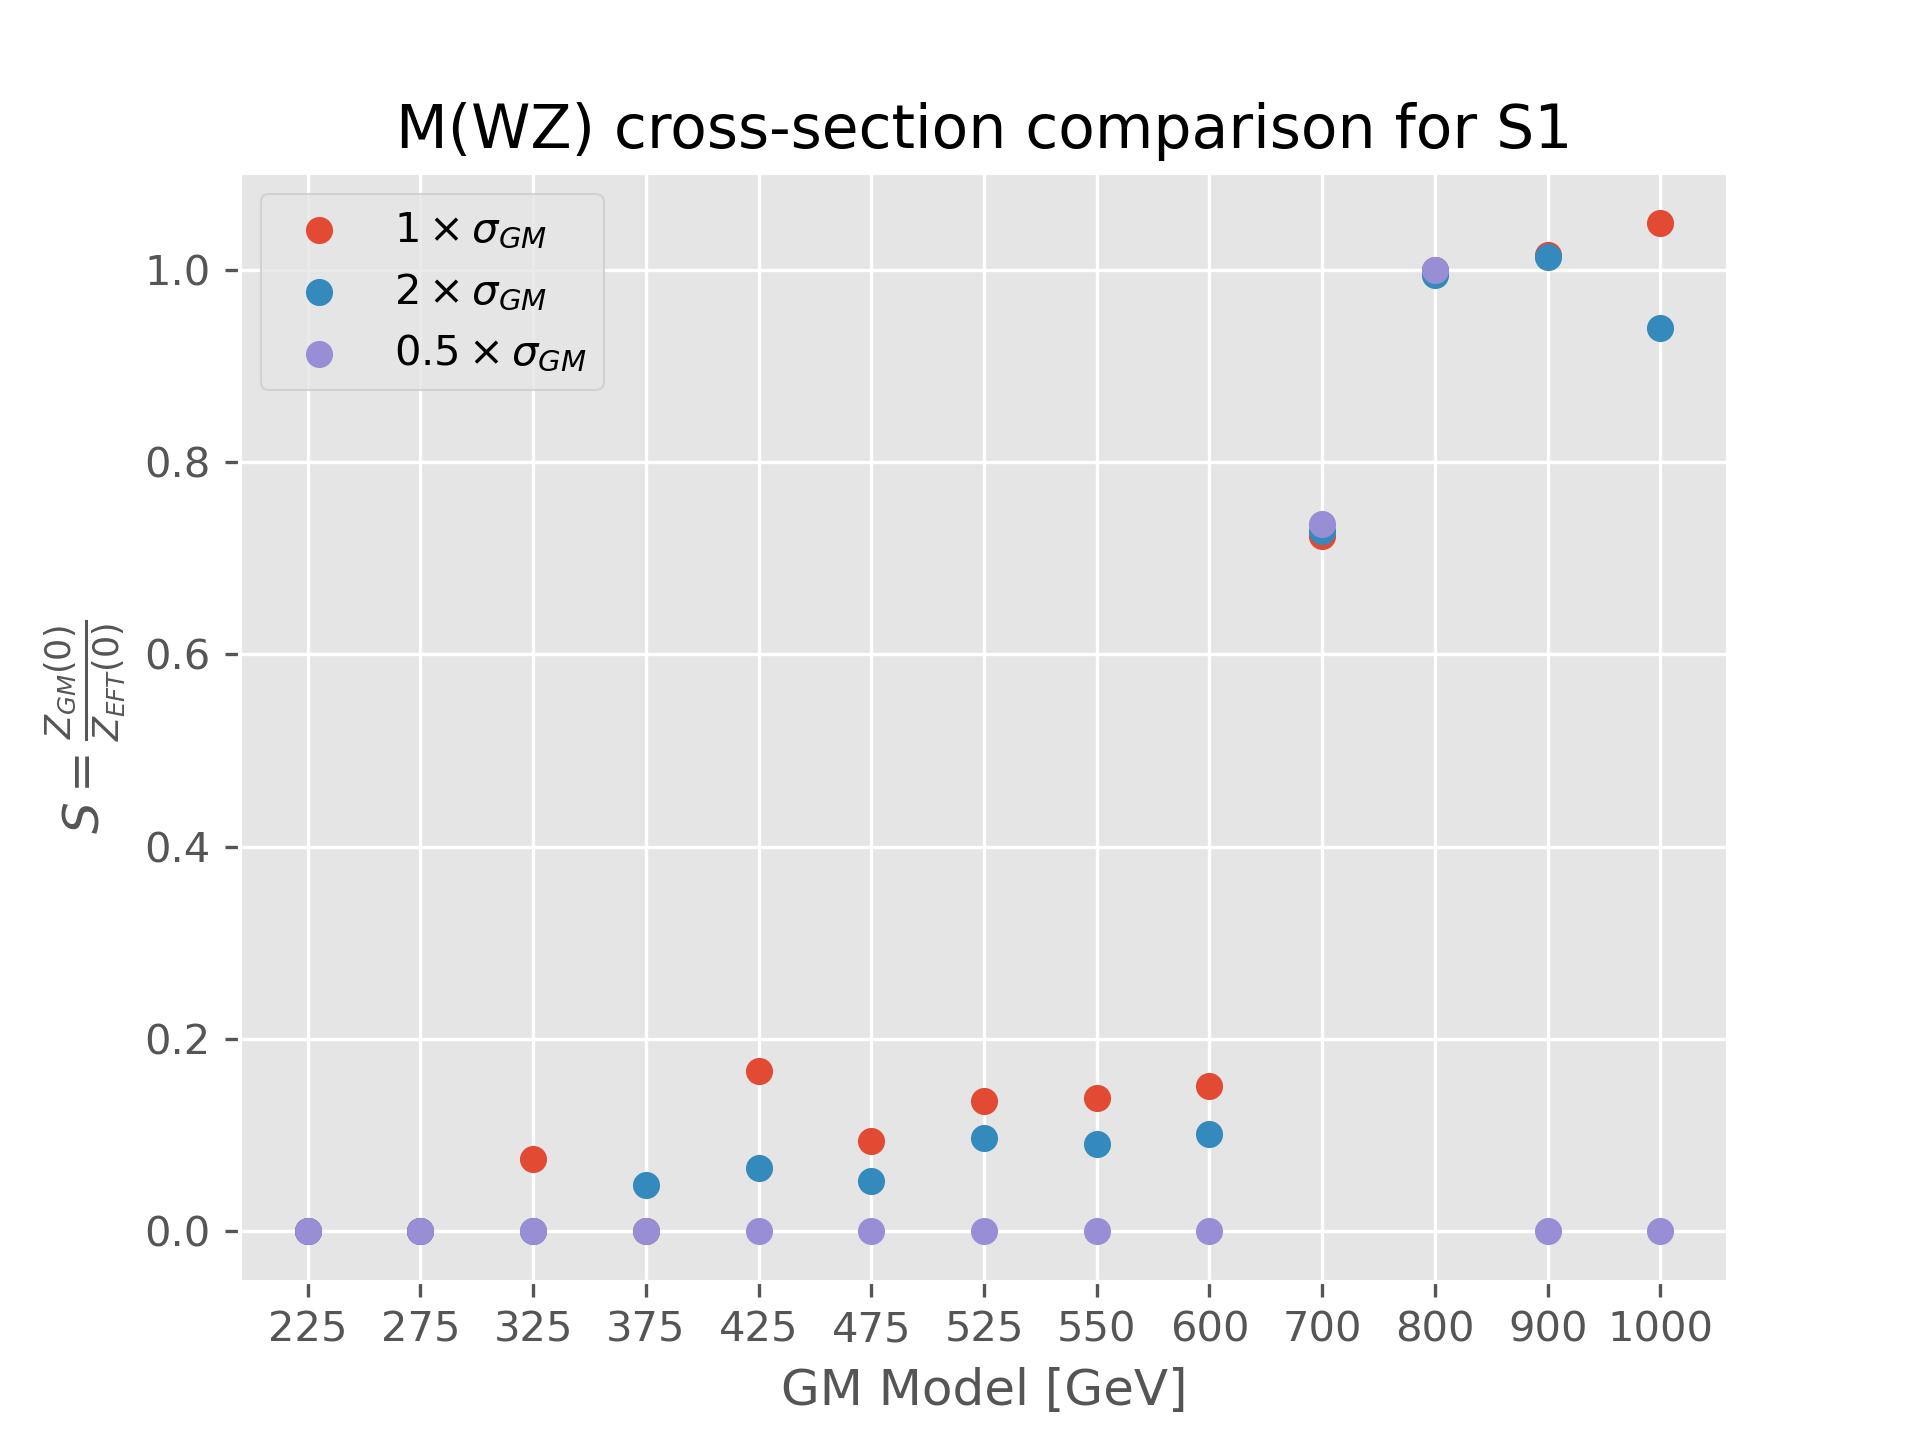
\includegraphics[width=\textwidth]{Plots/gm_relevanze/MWZ_comparision_S1.png}
        \caption{}
    \end{subfigure}
    \begin{subfigure}{0.45\textwidth}
        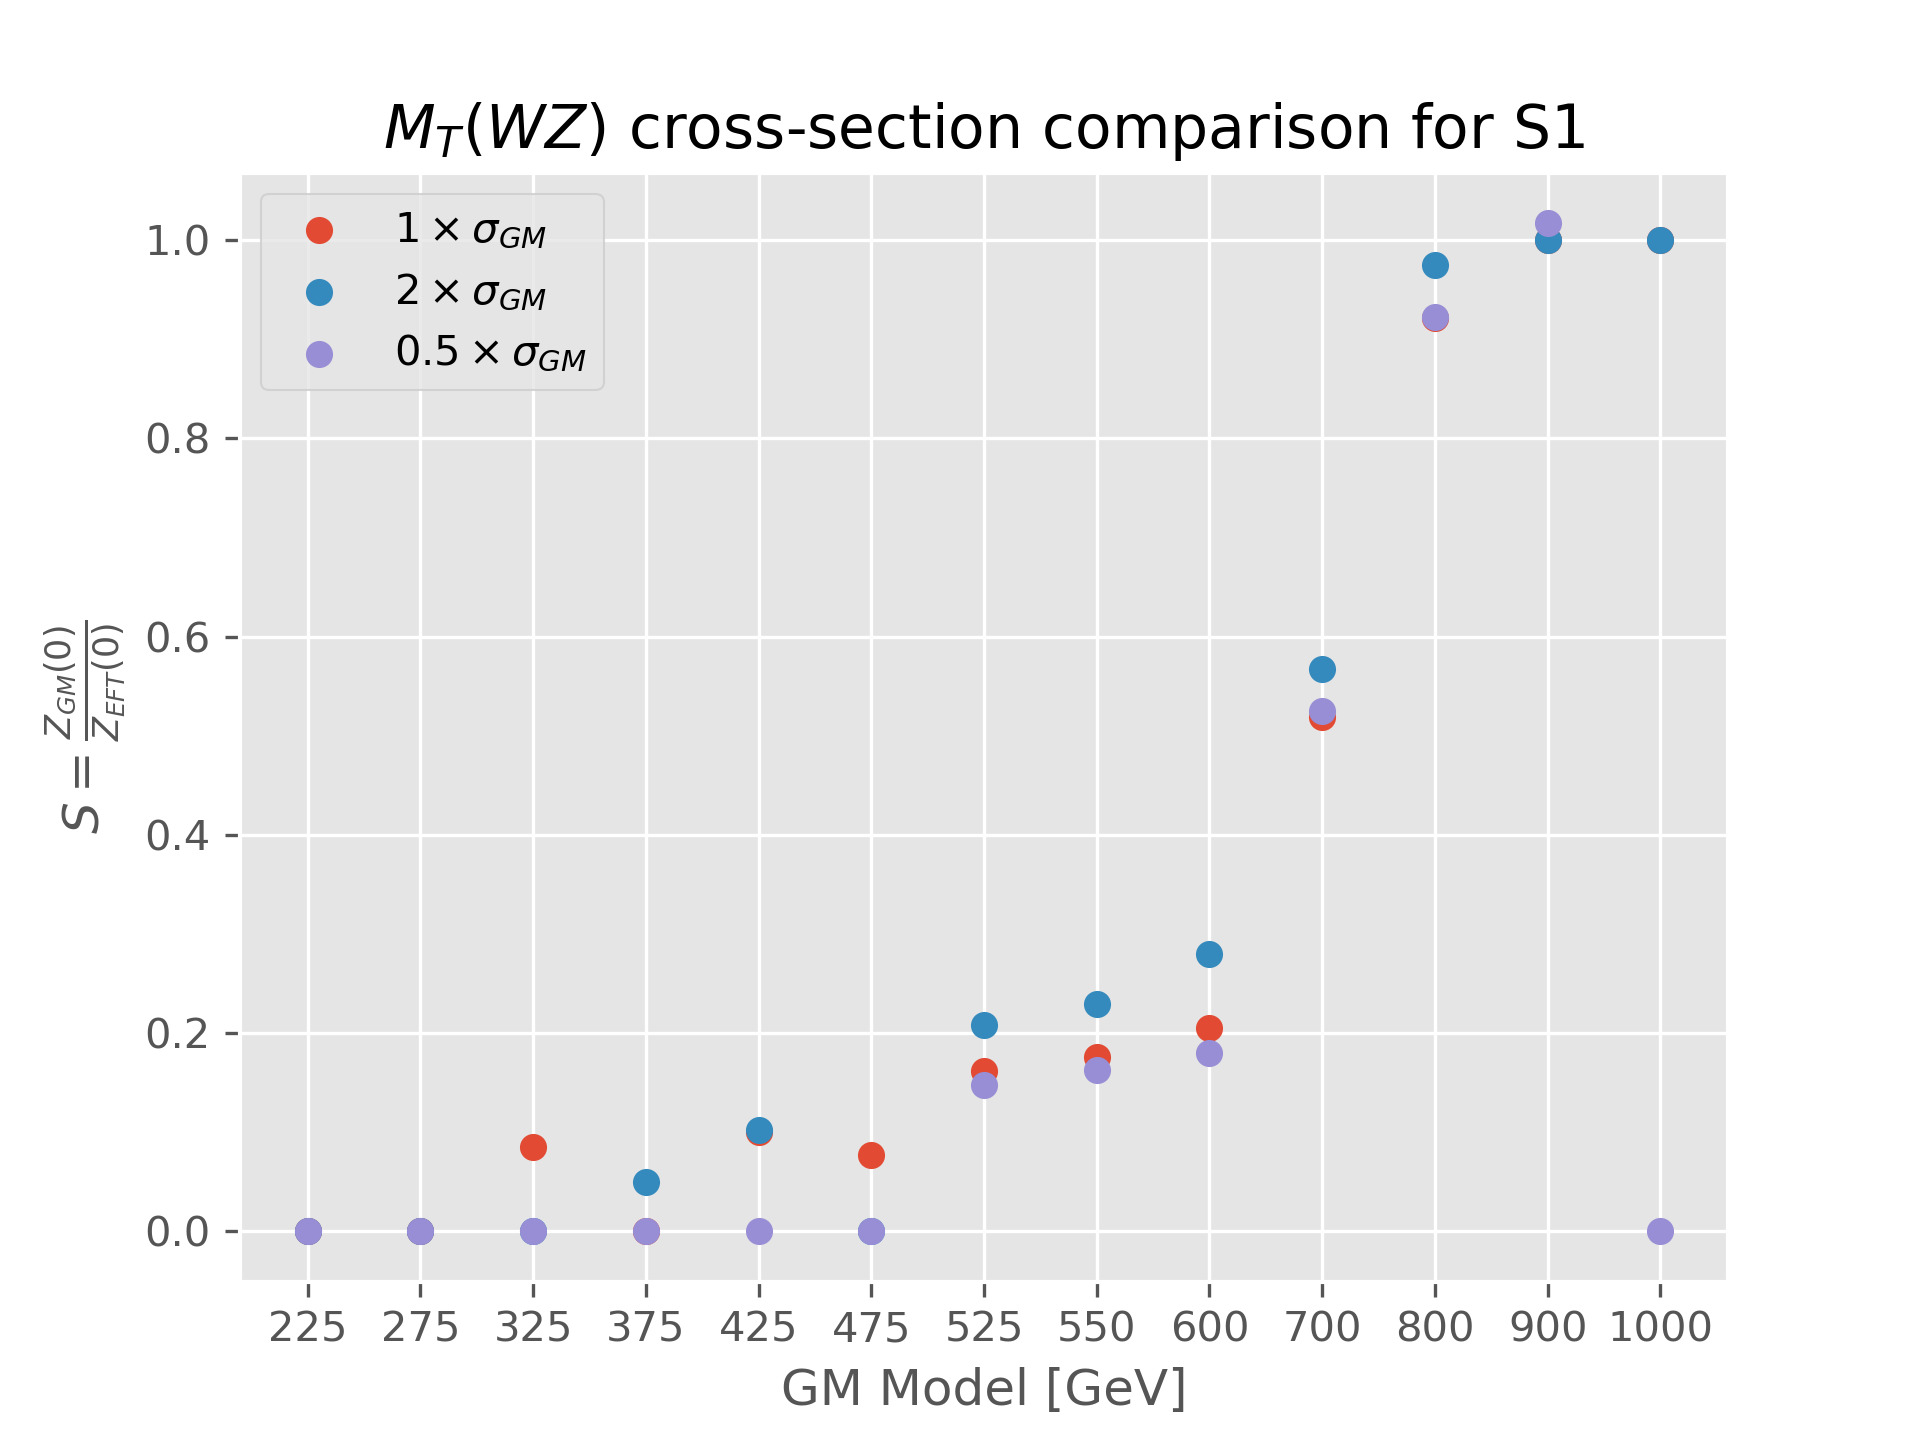
\includegraphics[width=\textwidth]{Plots/gm_relevanze/MTWZ_comparision_S1.png}
        \caption{}
    \end{subfigure}
    \caption{\textbf{a)} \acrshort{eft} coefficients significance for invariant Mass \textbf{b)} \acrshort{eft} coefficients significance for transverse Mass. The comparison for all operators is shown in \ref{sec:cross-section-comp}}
    \label{fig:corss-section-comparission}
\end{figure}

The 700 GeV sample has a significance of $0.7-0.8$ making it irrelevant for this analysis
but with the high dependence on the binning one may be able to get a significant result by optimizing the binning. The \acrshort{eft} limits for relevant resonance masses are shown in tabular \ref{tab:inv_mass_EFT_limits}. The limits for both extrema should be equivalent but the \acrshort{eft}Fun only expects one extremum when fitting
and therefore includes the second extremum in the $95\%$CL if the second extremum is to close to the first extremum.  In order to find both extrema the range from a minimal range to zero for the negative extremum and from zero to a positive minimal range.
The minimal range should leave space for the fit to find the best fit value. T0 doesn't show this behaviour which is likely caused by the larger uncertainties shown in \ref{fig:all_mwz_800} and \ref{fig:all_mtwz_800}.
A full set of all parameters and both invariant mass and transverse mass are shown in \ref{fig:all_mwz_800} and \ref{fig:all_mtwz_800} for an 800 GeV resonance as this is the resonance with the lowest energy and statistical significance. Other significant resonances are shown in the appendix \ref{sec:further_resonace}.
For the 1000 GeV resonance the coefficients T1, T0 in the invariant mass plot as well as M0, T0, T1 in the traverse mass plots could not be fitted as the cross-section is too small.



\begin{table}[h]
    \centering
    \begin{tabular}{ l c c c c c c }
        \multicolumn{7}{c}{ $M(WZ)$ }                                                                            \\
        Mass     & S1           & M0            & M1           & T0              & T1            & T2            \\
        \hline
        \multicolumn{7}{l}{ positive extrema }                                                                   \\
        800 GeV  & [89,129]     & [20,28.4]     & [29,42.4]    & [2.1,2.8]       & [1.4,2.01]    & [4.1,6.03]    \\
        900 GeV  & [-10,76.8]   & [1.1,17.2]    & [-0.41,25.3] & no extrema      & [-0.057,1.18] & [0.035,3.56]  \\
        1000 GeV & [-447,71.7]  & [281,16.2]    & [-207,23.6]  & no extrema      & [-0.5,1.1]    & [-8.2,3.32]   \\
        \multicolumn{7}{l}{ negative extrema }                                                                   \\
        800 GeV  & [-130,-90.4] & [-27,-18.4]   & [-43,-29.6]  & [-1.9,-1.11]    & [-2.1,-1.48]  & [-6.3,-4.37]  \\
        900 GeV  & [-78,248]    & [-16, -0.115] & [-26,0.329]  & [-0.89,0.109]   & [-1.3,0.0591] & [-3.8,0.186]  \\
        1000 GeV & [-73,1096]   & [-15,5.52]    & [-24,9.92]   & [-0.81,0.231]   & [-1.2,14.3]   & [-3.6,1.04]   \\
        \hline
        \multicolumn{7}{c}{}                                                                                     \\
        \multicolumn{7}{c}{ $M_{T}(WZ)$ }                                                                        \\
        Mass     & S1           & M0            & M1           & T0              & T1            & T2            \\
        \hline
        \multicolumn{7}{l}{ positive extrema }                                                                   \\
        800 GeV  & [75,113]     & [16,24.2]     & [24,36.2]    & no extrema      & [1.1,1.73]    & [3.2,5.0]     \\
        900 GeV  & [15,68.4]    & [3.4,14.8]    & [4.9,22.2]   & no extrema      & [0.22,1.06]   & [0.6,3.06]    \\
        1000 GeV & [-19,64.7]   & [220.45,14]   & [-23,21]     & no extrema      & [-0.33,1.0]   & [-0.45,2.89]  \\
        \multicolumn{7}{l}{ negative extrema }                                                                   \\
        800 GeV  & [-115,-76.3] & [-24,-15.5]   & [-36,-23.8]  & [-1.5,-0.792]   & [-1.5,-0.792] & [-5.2,-3.41]  \\
        900 GeV  & [-70,-16.4]  & [-14,-2.99]   & [-22,-4.97]  & [-0.77,-0.0389] & [-1.1,-0.256] & [-3.3,-0.798] \\
        1000 GeV & [-66,78.6]   & [-14,6.69]    & [-21,82.6]   & [-0.71,0.0189]  & [-1.0,0.97]   & [-3.1,37.9]   \\
        \hline
    \end{tabular}

    \caption{Invariant mass lower and upper $95\%$ confidence level limits for a fit with linear and quadratic operators in WZ with all other aQGC parameters set to zero}
    \label{tab:inv_mass_EFT_limits}

\end{table}

\begin{figure}[h]

    \centering
    \begin{subfigure}{0.3\textwidth}
        \includegraphics[width=\textwidth]{Plots/ALL_MWZ_final/GM_H5_800/S1/2022-05-07/VBSSR/all_VV_MWZ_vbs.pdf}
    \end{subfigure}
    \begin{subfigure}{0.3\textwidth}
        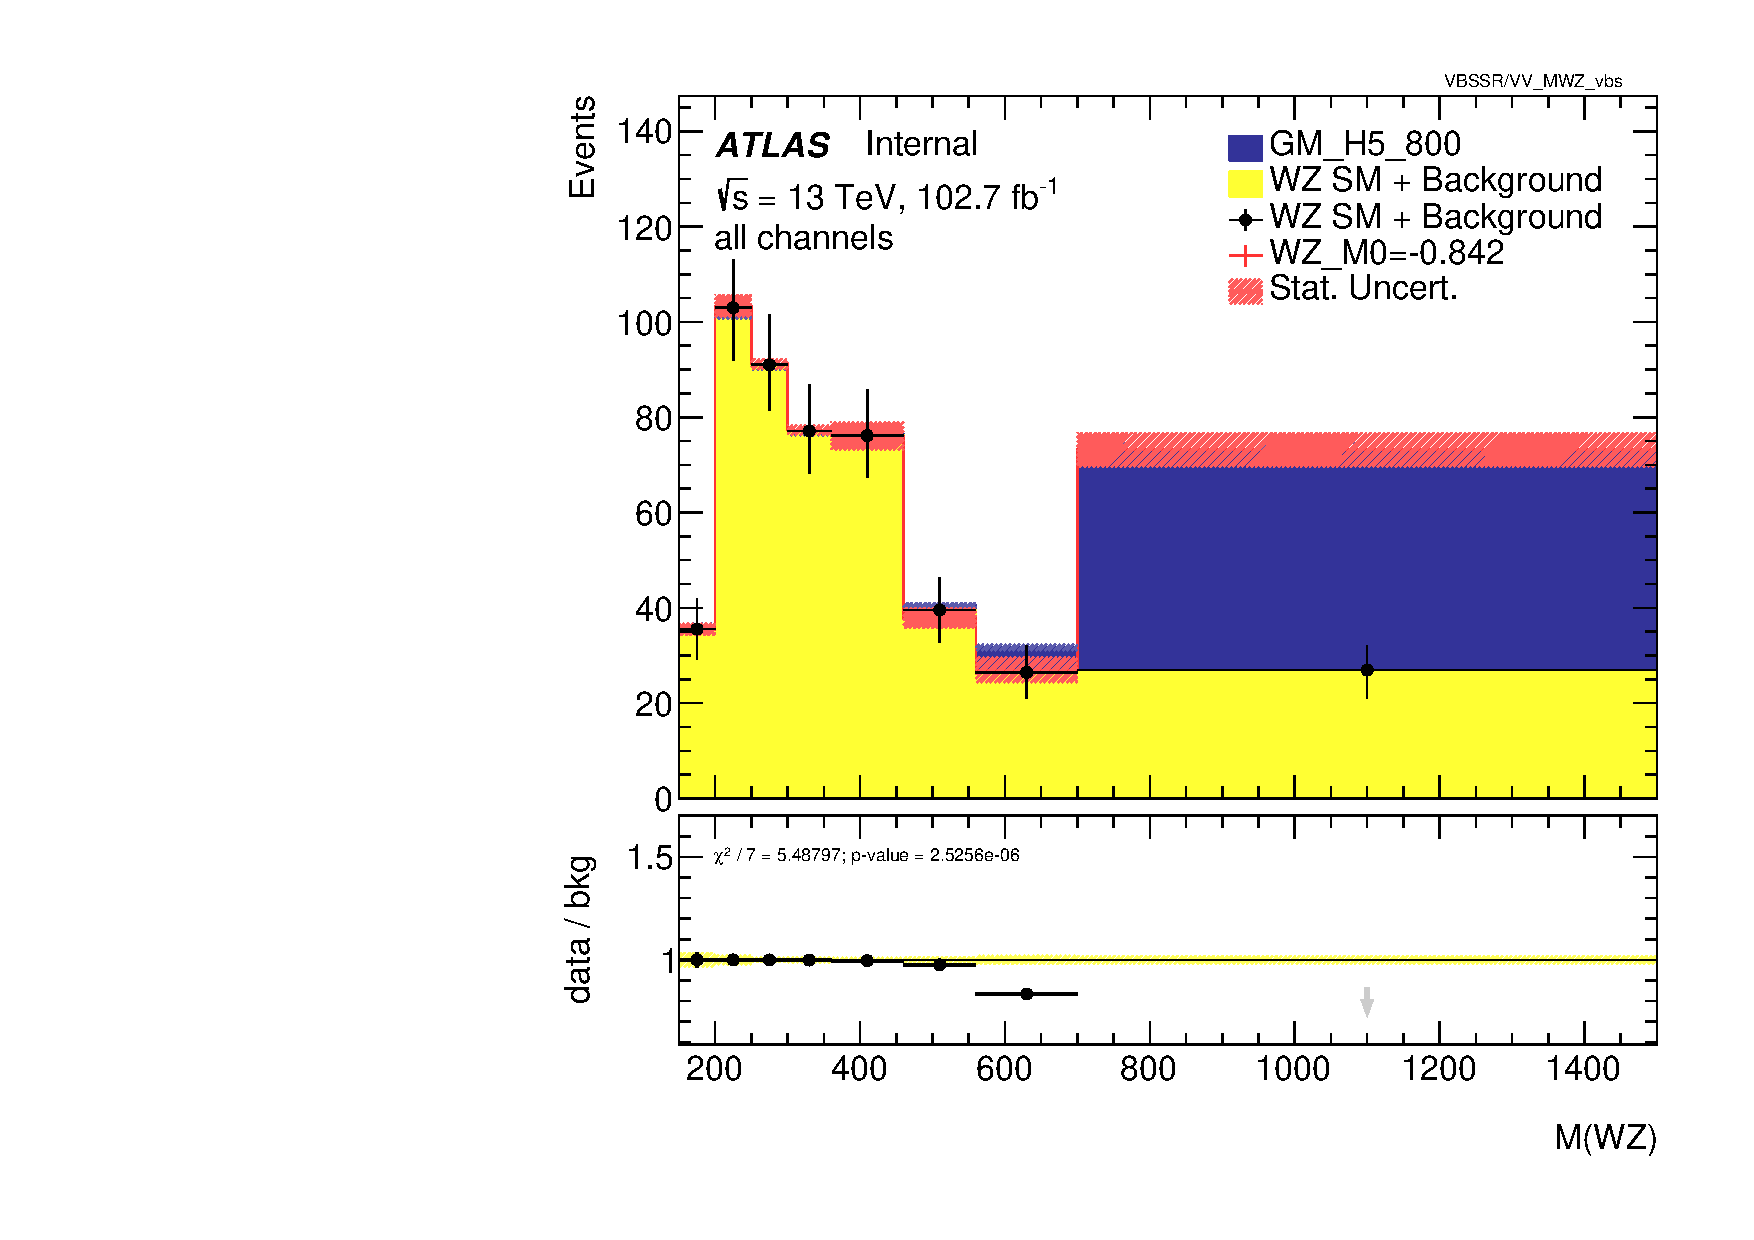
\includegraphics[width=\textwidth]{Plots/ALL_MWZ_final/GM_H5_800/M0/2022-05-07/VBSSR/all_VV_MWZ_vbs.pdf}
    \end{subfigure}
    \begin{subfigure}{0.3\textwidth}
        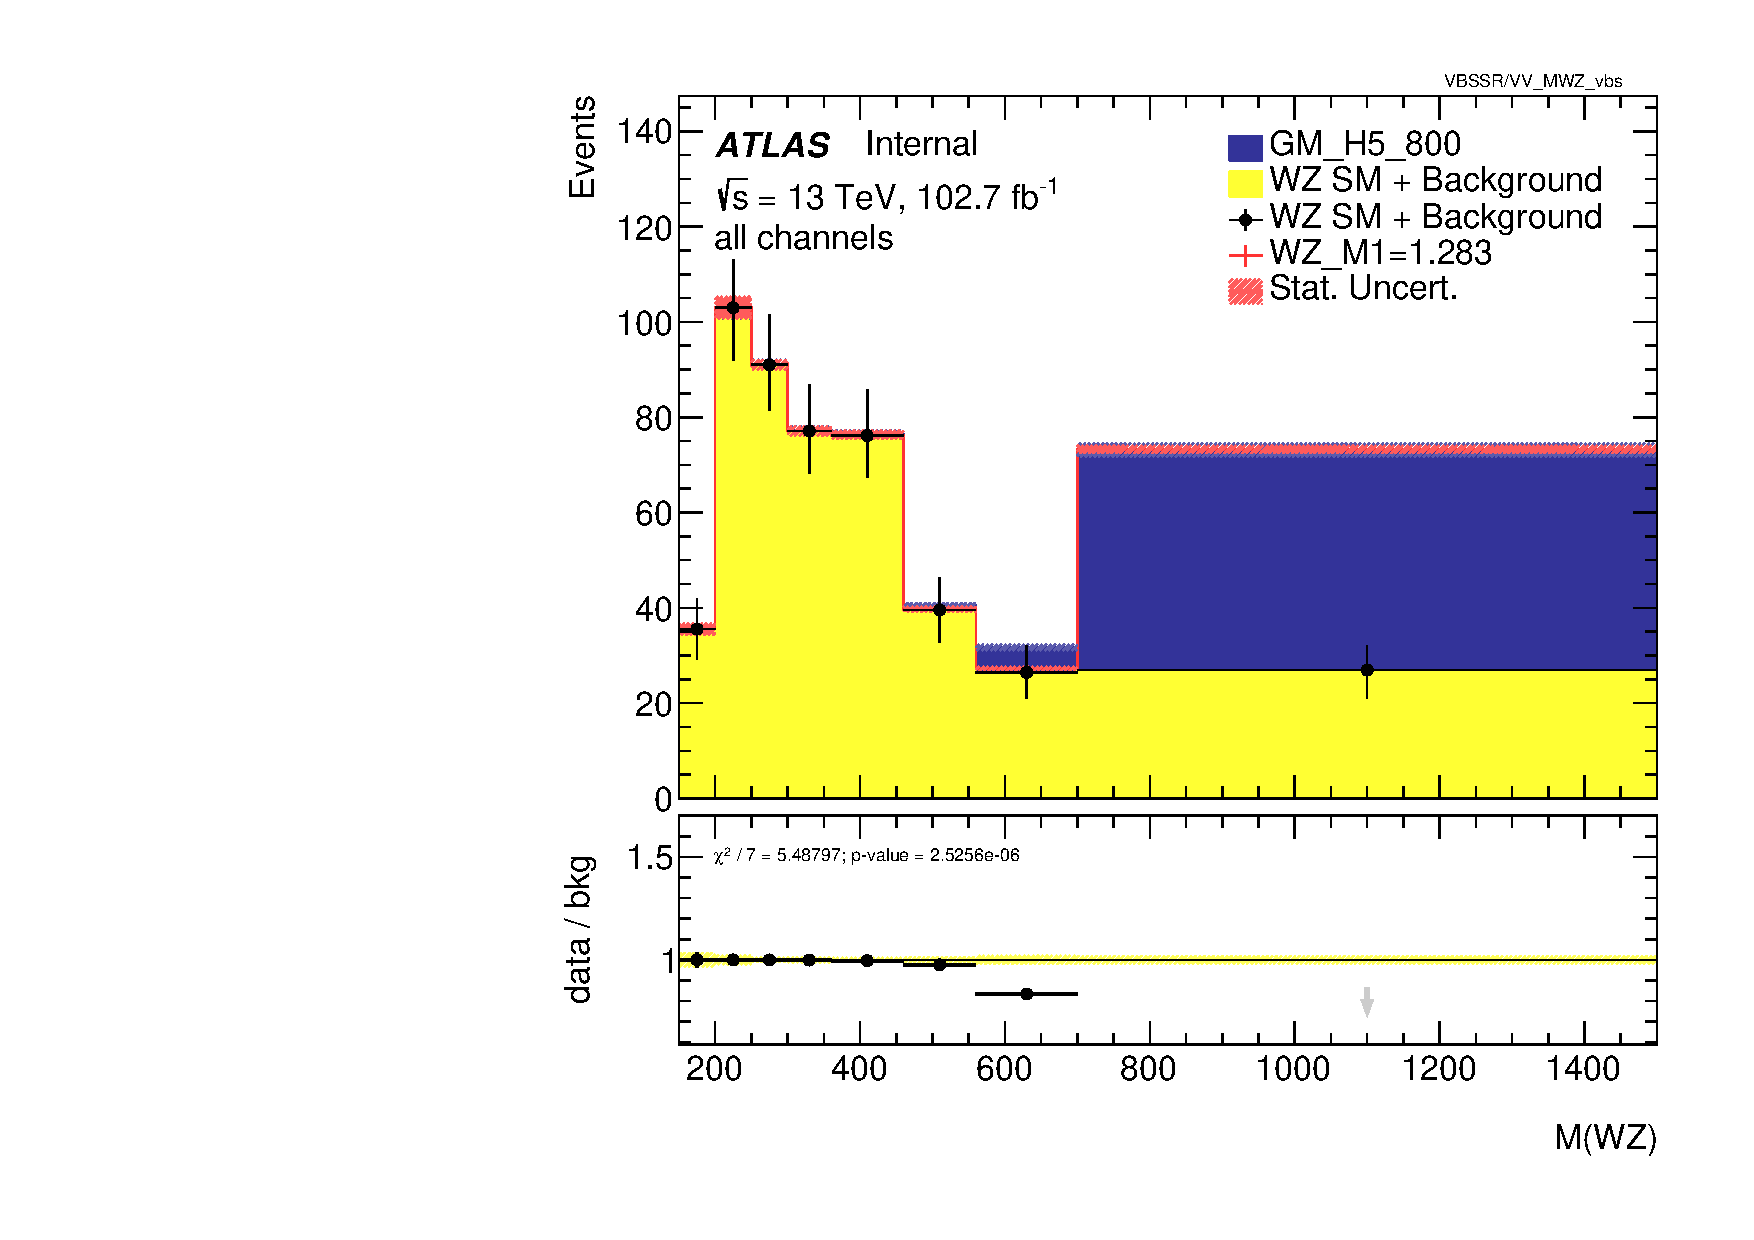
\includegraphics[width=\textwidth]{Plots/ALL_MWZ_final/GM_H5_800/M1/2022-05-07/VBSSR/all_VV_MWZ_vbs.pdf}
    \end{subfigure}
    \begin{subfigure}{0.3\textwidth}
        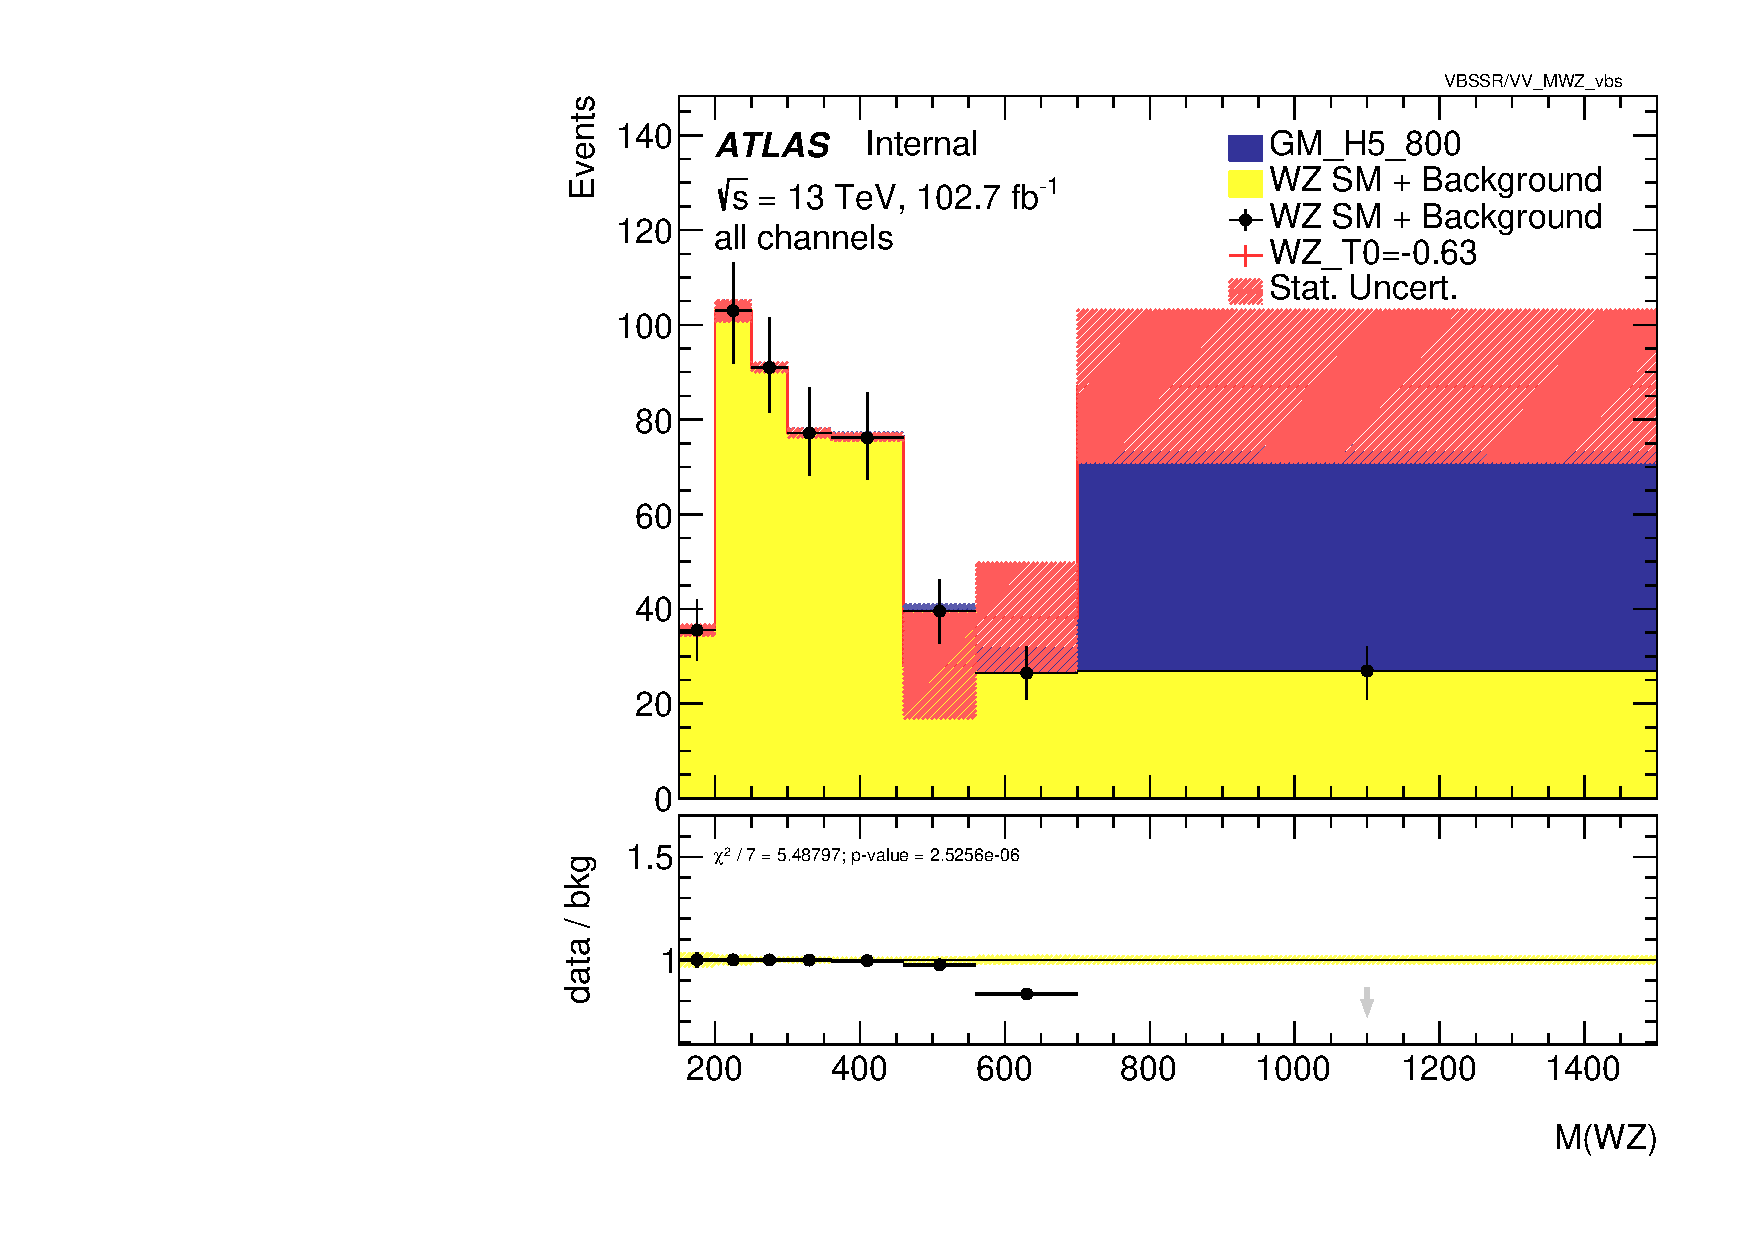
\includegraphics[width=\textwidth]{Plots/ALL_MWZ_final/GM_H5_800/T0/2022-05-07/VBSSR/all_VV_MWZ_vbs.pdf}
    \end{subfigure}
    \begin{subfigure}{0.3\textwidth}
        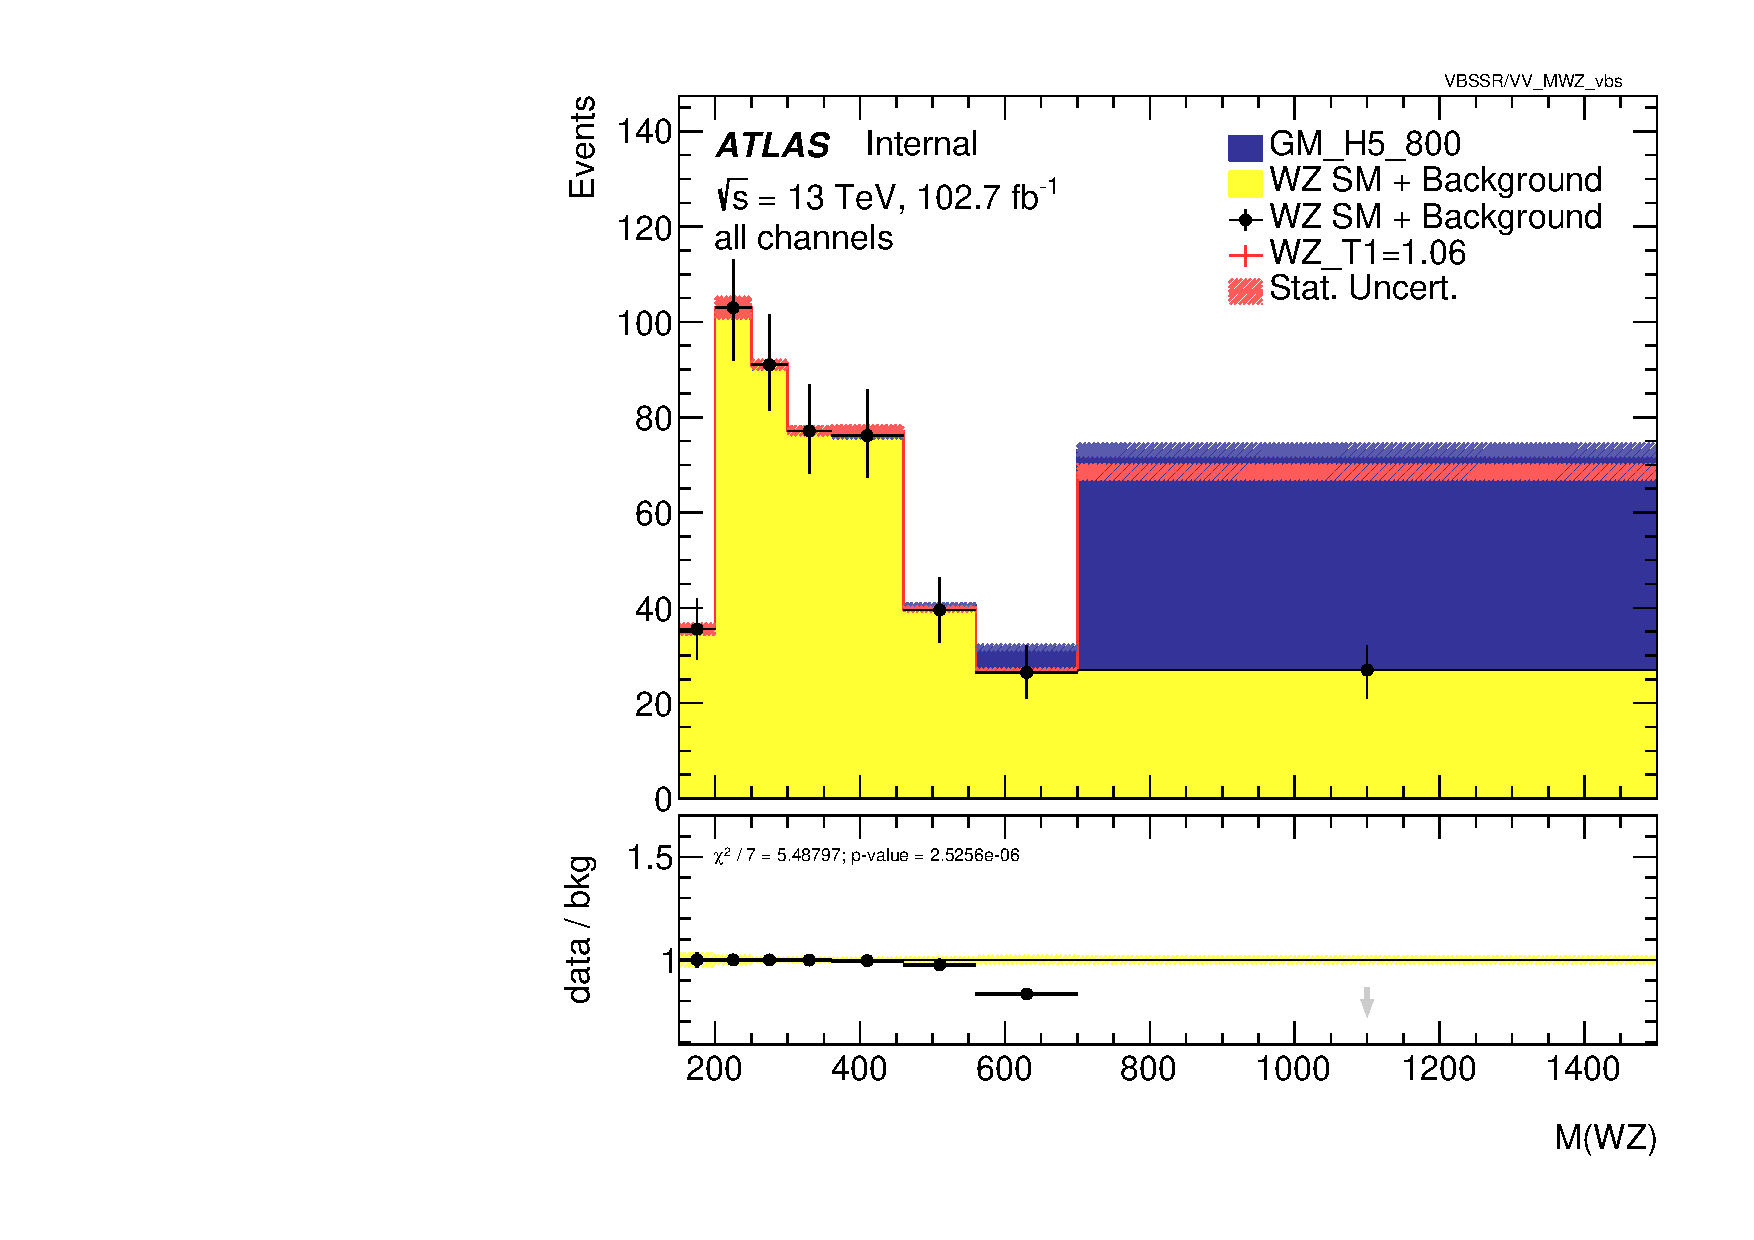
\includegraphics[width=\textwidth]{Plots/ALL_MWZ_final/GM_H5_800/T1/2022-05-07/VBSSR/all_VV_MWZ_vbs.pdf}
    \end{subfigure}
    \begin{subfigure}{0.3\textwidth}
        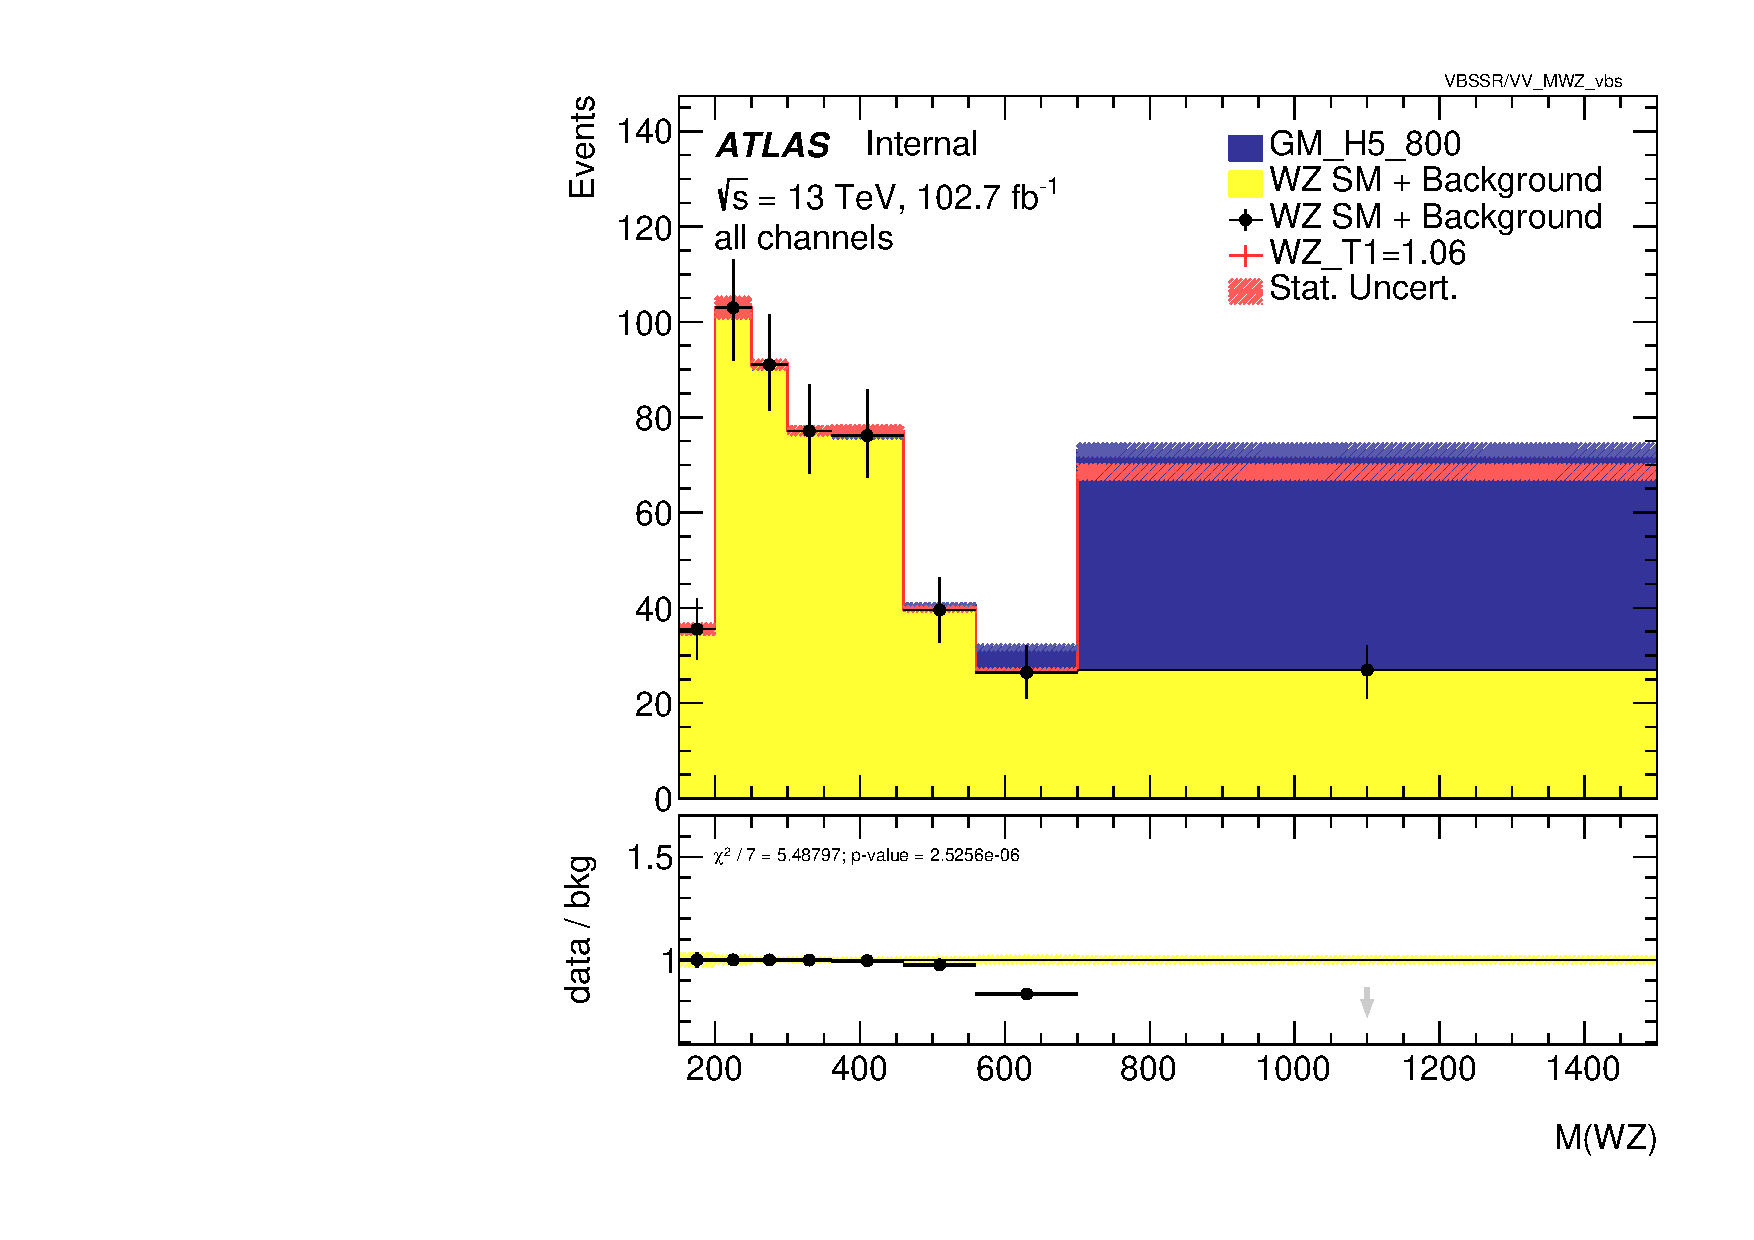
\includegraphics[width=\textwidth]{Plots/ALL_MWZ_final/GM_H5_800/T1/2022-05-07/VBSSR/all_VV_MWZ_vbs.pdf}
    \end{subfigure}

    \caption{Invariant mass for parameters S1, M0, M1, T0, T1, T2 with best fit value for 800 GeV resonance}
    \label{fig:all_mwz_800}
\end{figure}

\begin{figure}[h]

    \centering
    \begin{subfigure}{0.3\textwidth}
        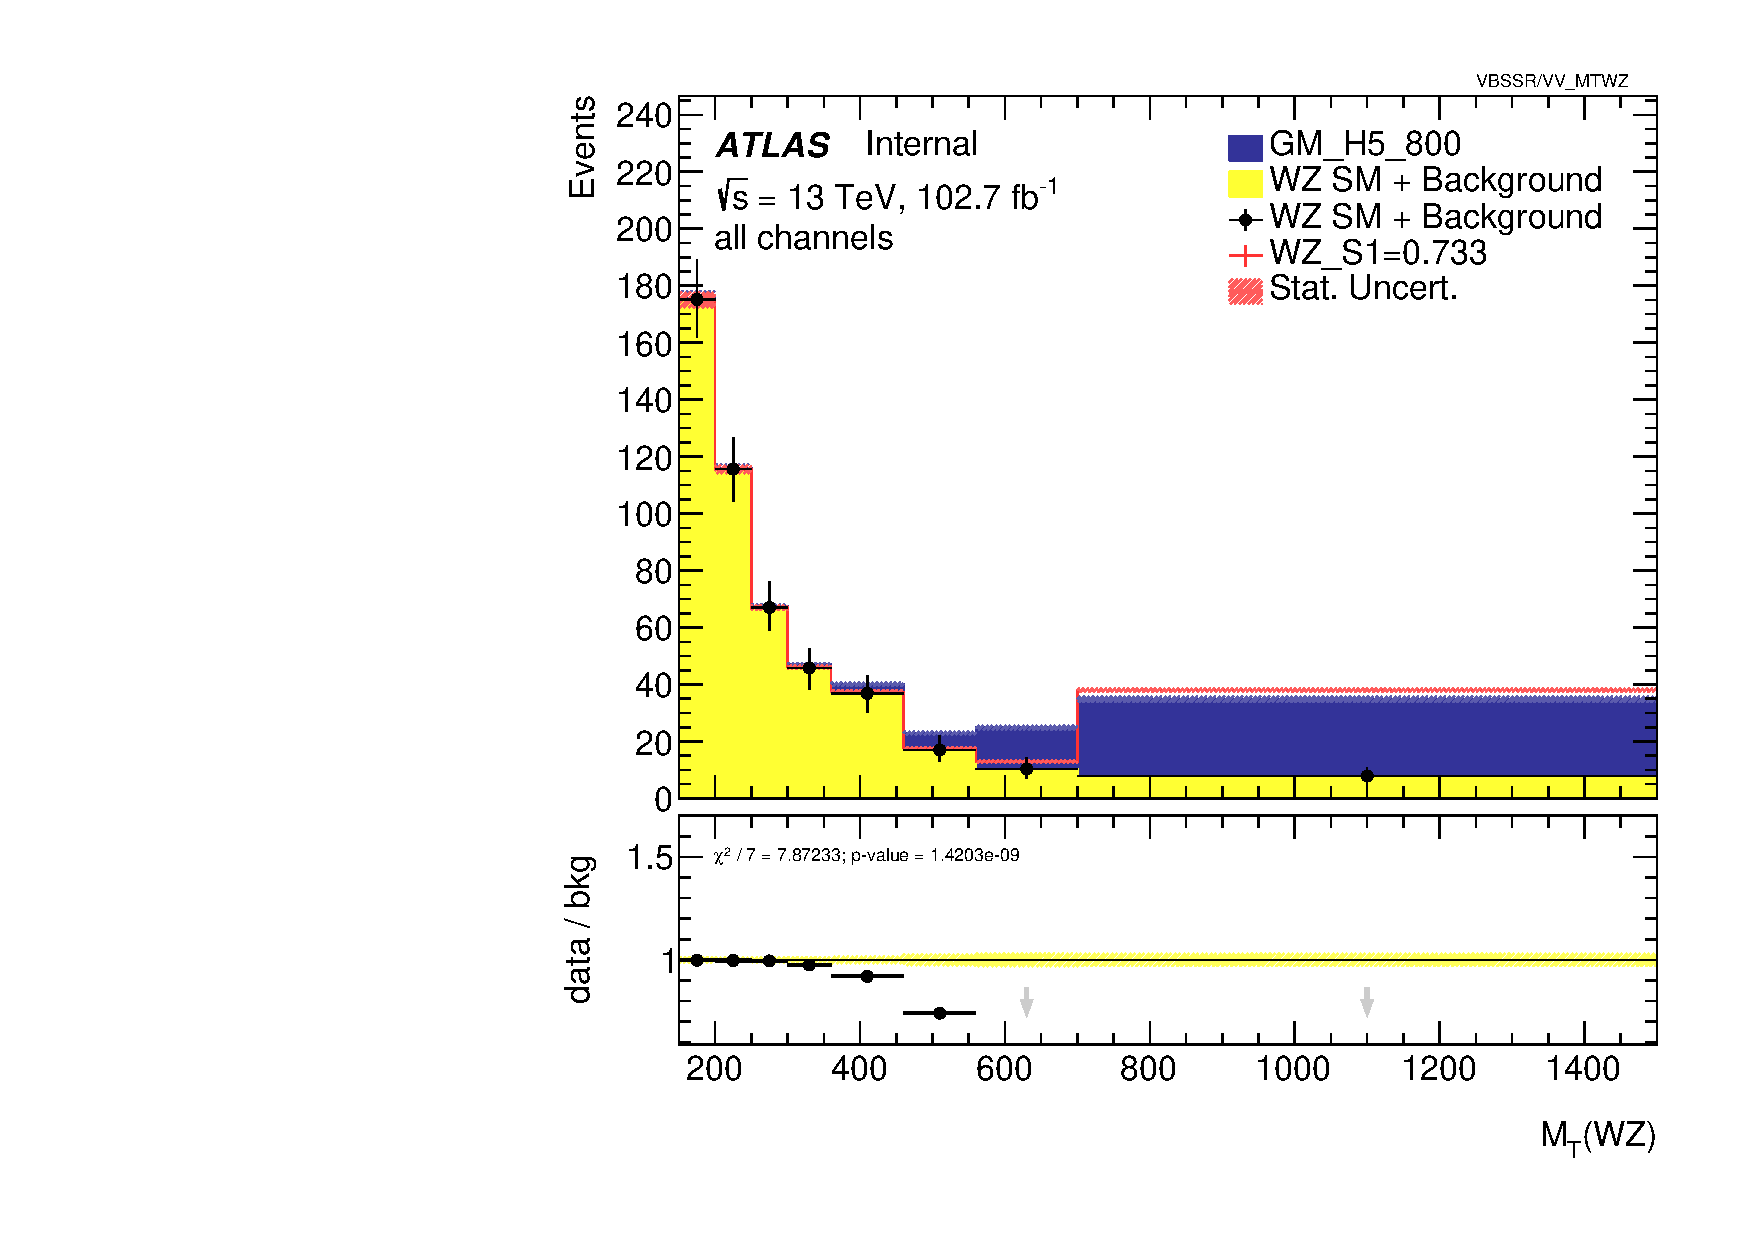
\includegraphics[width=\textwidth]{Plots/ALL_MTWZ_final/GM_H5_800/S1/2022-05-07/VBSSR/all_VV_MTWZ.pdf}
    \end{subfigure}
    \begin{subfigure}{0.3\textwidth}
        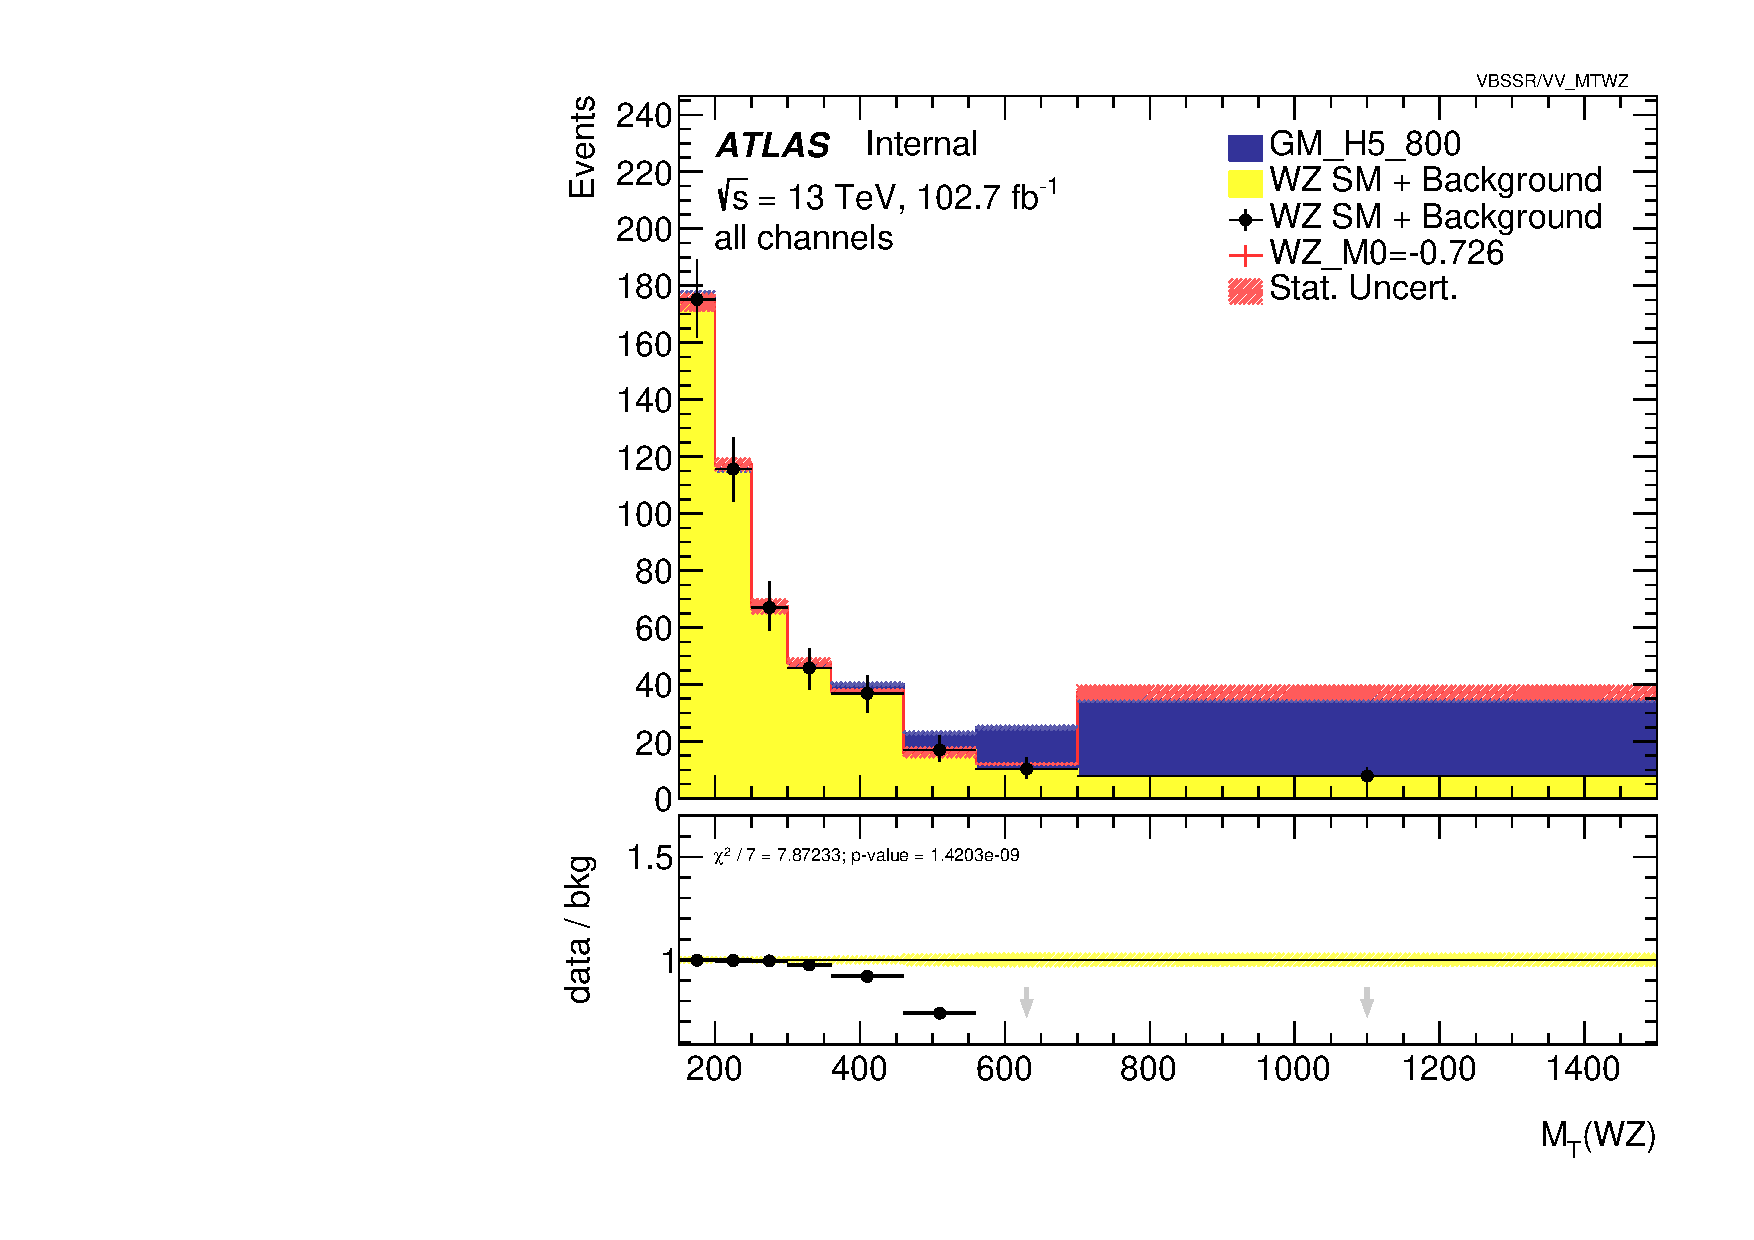
\includegraphics[width=\textwidth]{Plots/ALL_MTWZ_final/GM_H5_800/M0/2022-05-07/VBSSR/all_VV_MTWZ.pdf}
    \end{subfigure}
    \begin{subfigure}{0.3\textwidth}
        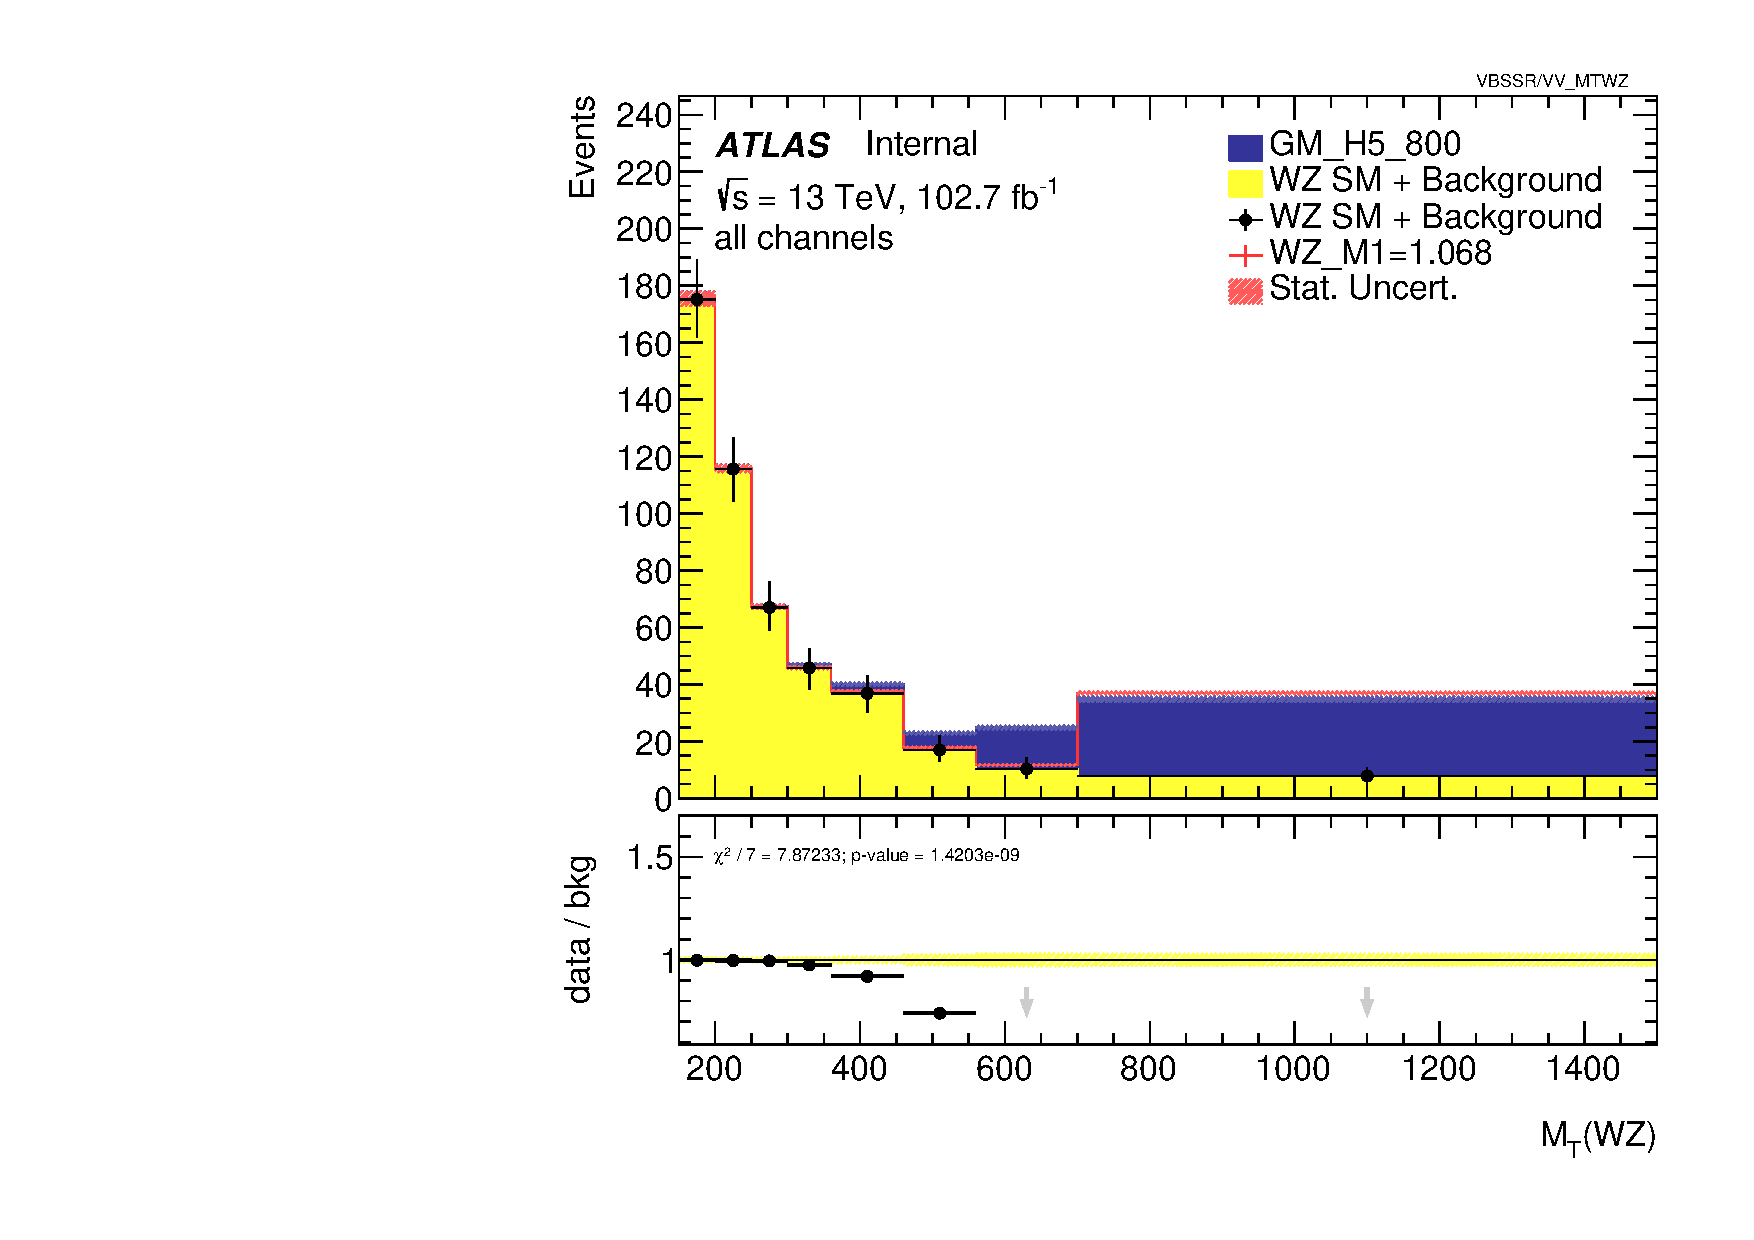
\includegraphics[width=\textwidth]{Plots/ALL_MTWZ_final/GM_H5_800/M1/2022-05-07/VBSSR/all_VV_MTWZ.pdf}
    \end{subfigure}
    \begin{subfigure}{0.3\textwidth}
        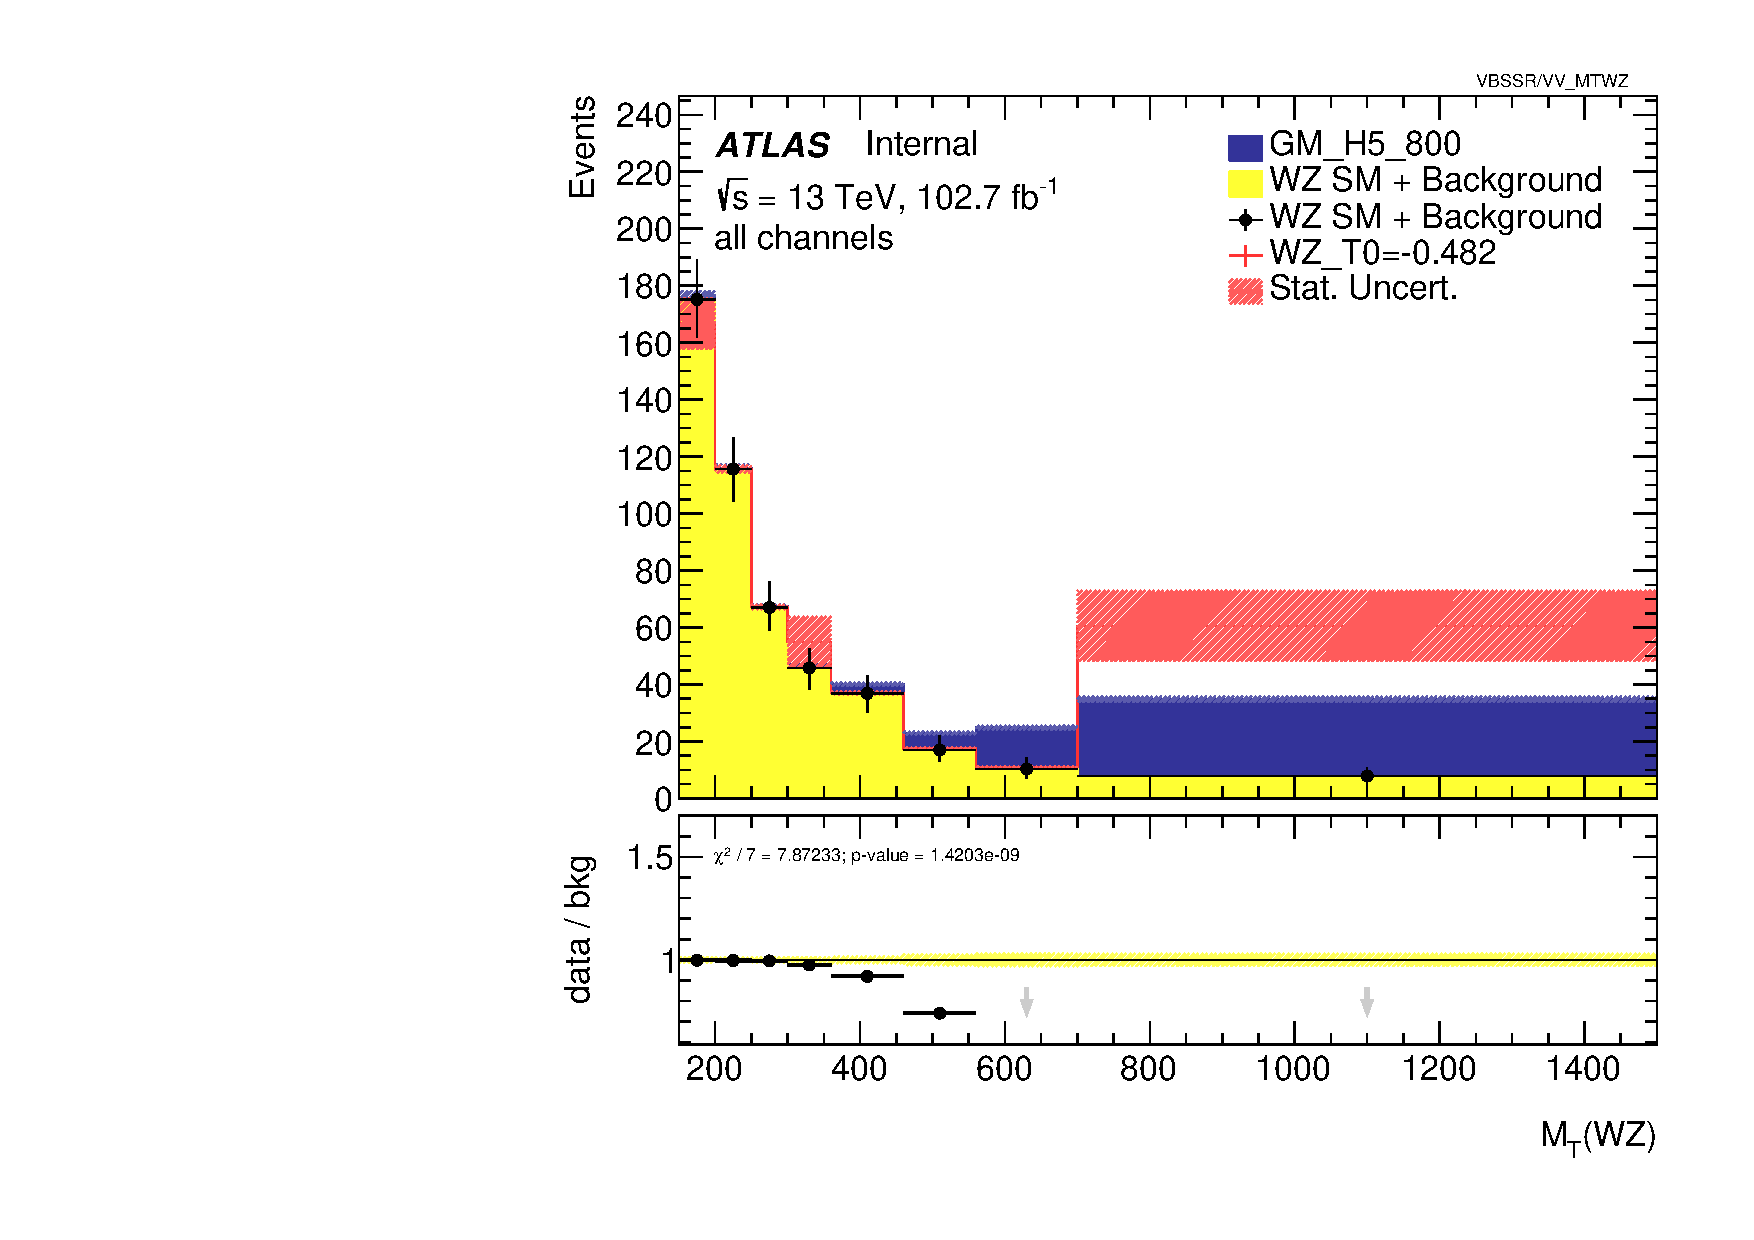
\includegraphics[width=\textwidth]{Plots/ALL_MTWZ_final/GM_H5_800/T0/2022-05-07/VBSSR/all_VV_MTWZ.pdf}
    \end{subfigure}
    \begin{subfigure}{0.3\textwidth}
        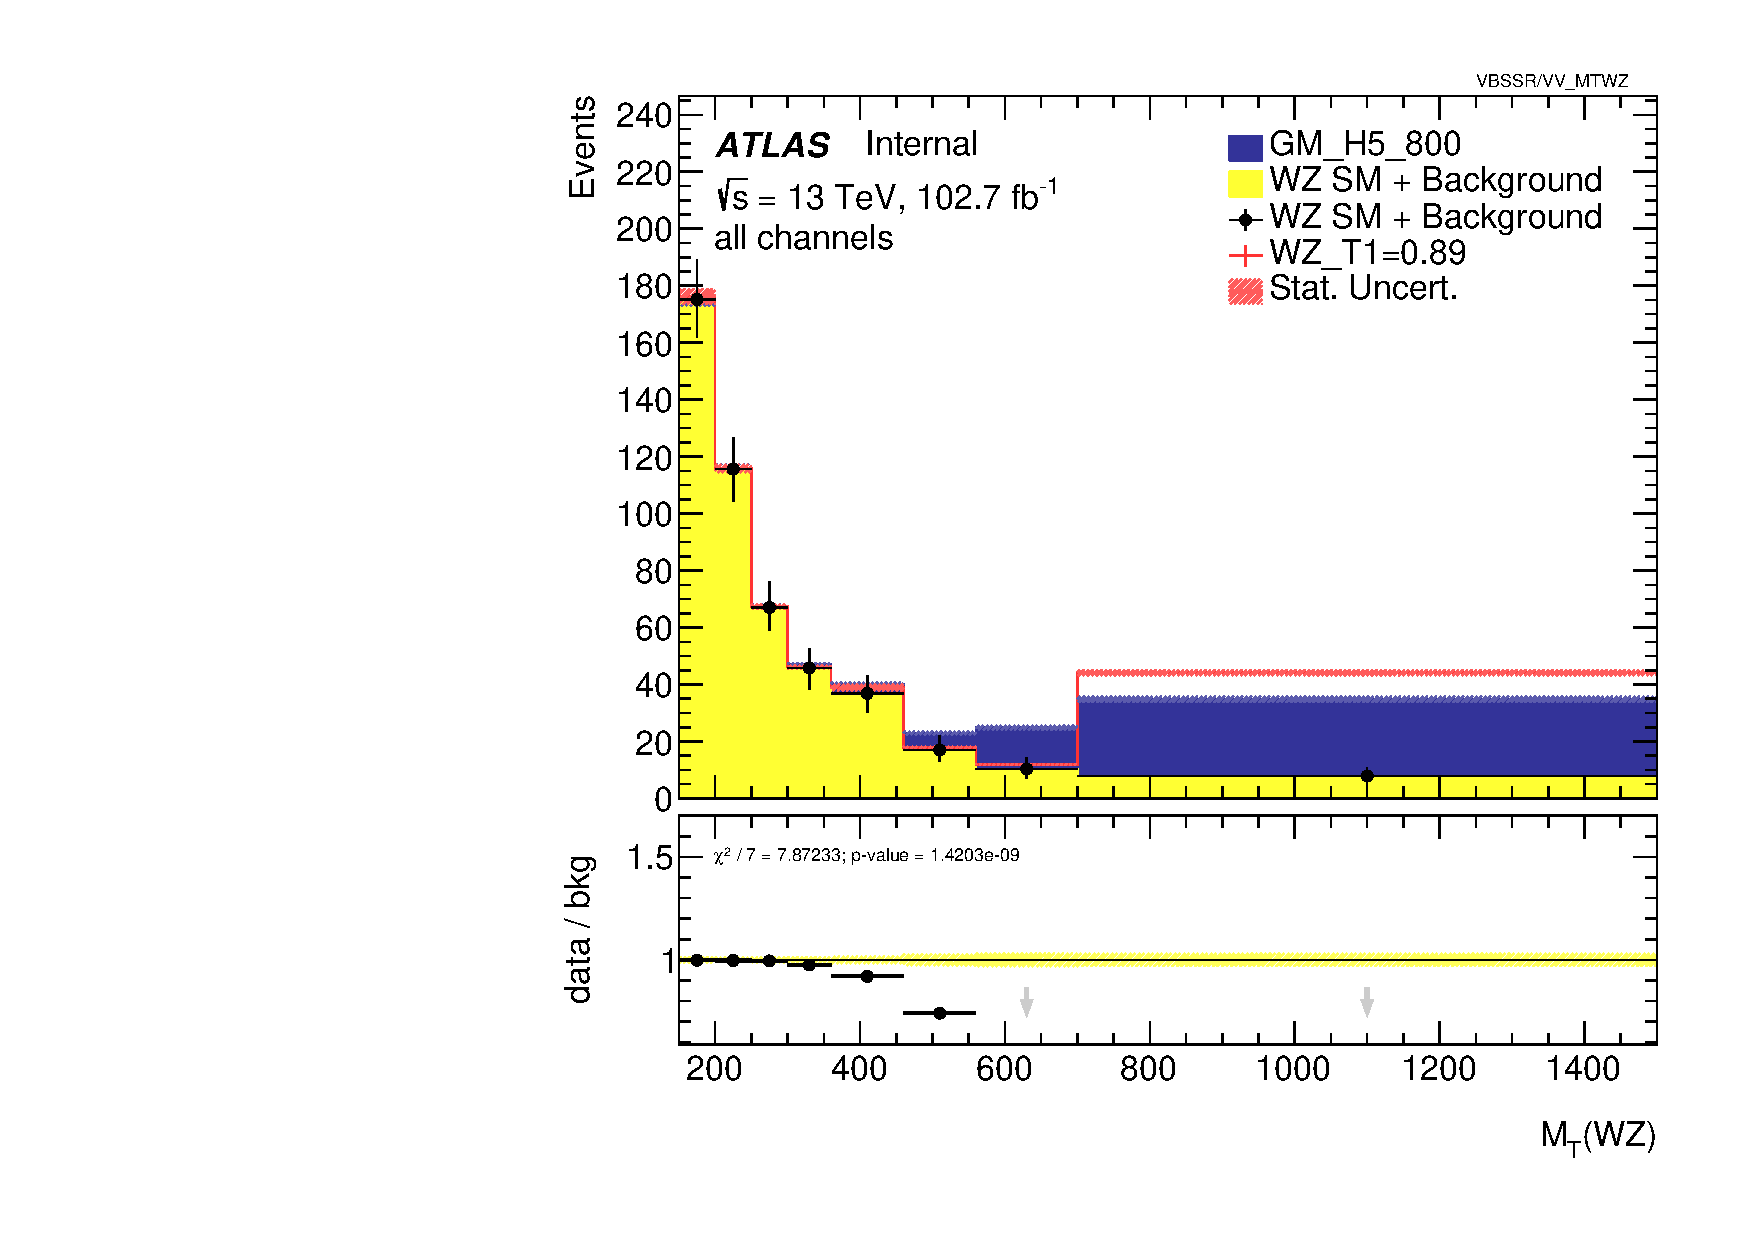
\includegraphics[width=\textwidth]{Plots/ALL_MTWZ_final/GM_H5_800/T1/2022-05-07/VBSSR/all_VV_MTWZ.pdf}
    \end{subfigure}
    \begin{subfigure}{0.3\textwidth}
        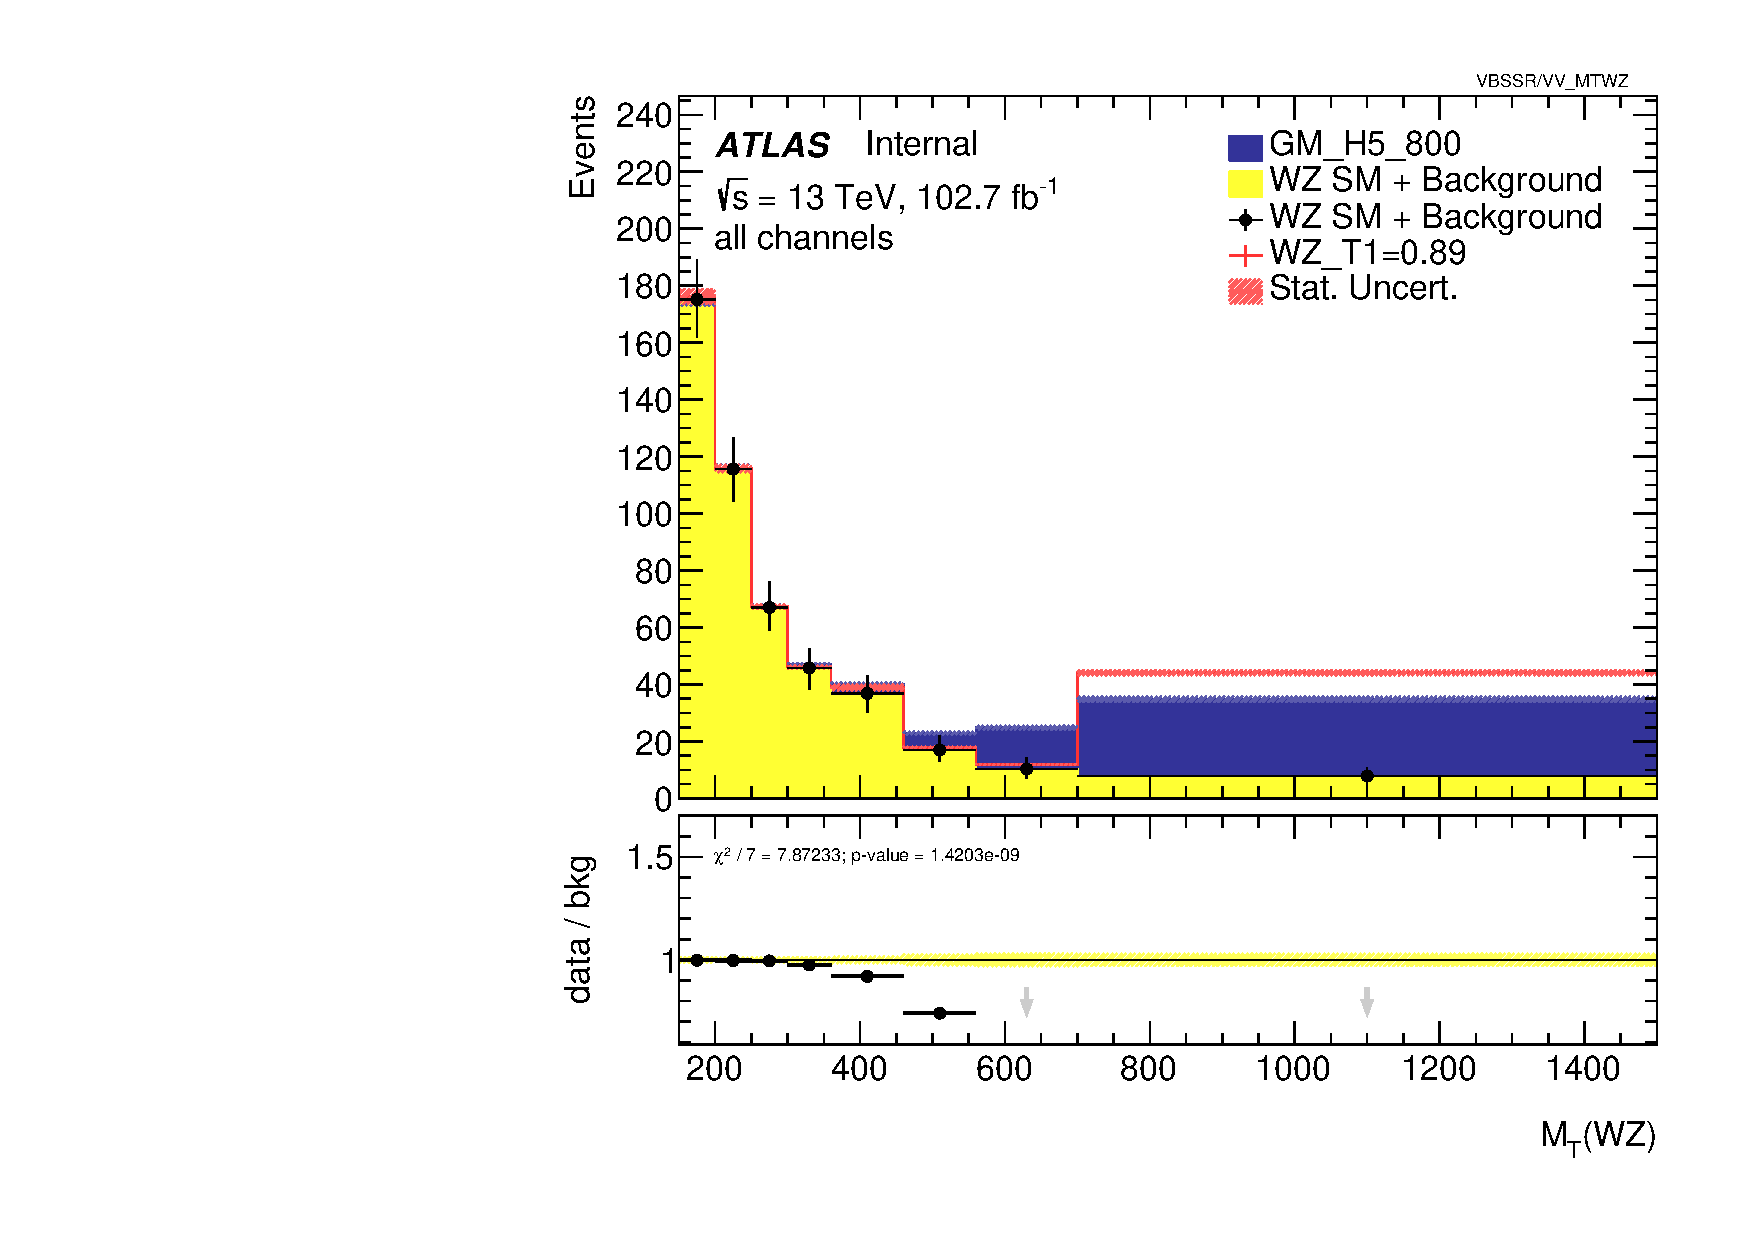
\includegraphics[width=\textwidth]{Plots/ALL_MTWZ_final/GM_H5_800/T1/2022-05-07/VBSSR/all_VV_MTWZ.pdf}
    \end{subfigure}

    \caption{transverse mass for parameters S1, M0, M1, T0, T1, T2 with best fit value for 800 GeV resonance}
    \label{fig:all_mtwz_800}
\end{figure}


\end{document}